\documentclass[11pt,a4paper]{article}

\usepackage[T1]{fontenc}
\usepackage[utf8]{inputenc}
\usepackage{lmodern}
\usepackage[magyar]{babel}
\usepackage{amsmath,amssymb,amsthm}
\usepackage{geometry}
\geometry{margin=2.3cm}
\usepackage{longtable}
\usepackage{booktabs}
\usepackage{array}
\usepackage{tikz}
\usetikzlibrary{arrows.meta,positioning,calc,decorations.pathreplacing,patterns,
  angles,quotes,shapes.geometric,shapes.misc,fit,backgrounds,matrix,trees}
\usepackage{hyperref}
\hypersetup{colorlinks=true,linkcolor=blue!50!black,urlcolor=blue!50!black}
\usepackage{enumitem}
\usepackage{caption}

\newcommand{\lean}[1]{\texttt{\small #1}}
\newcommand{\R}{\mathbb{R}}
\newcommand{\N}{\mathbb{N}}
\newcommand{\Z}{\mathbb{Z}}
\newcommand{\Q}{\mathbb{Q}}
\newcommand{\eps}{\varepsilon}

\theoremstyle{definition}
\newtheorem{rajz}{Rajz}[section]
\newtheorem{fogas}{Fogás}[section]

\tikzset{
  pont/.style={circle,fill,inner sep=1.2pt},
  ures/.style={circle,draw,fill=white,inner sep=1.2pt},
  nyil/.style={-{Latex[length=2mm]}},
  dob/.style={draw,rounded corners,inner sep=3pt,align=center,font=\small},
  seg/.style={thick},
  hal/.style={draw,thick},
}

\title{\textbf{Rajzos gondolkodás a Kalkulus 1.\ gyakorlófeladatokhoz}\\[2mm]
\large Hogyan találjuk meg és ellenőrizzük a bizonyításokat ceruzával:
Venn-diagramok, tablófák, számegyenes- és koordináta-rajzok, pókháló, kommutatív diagramok}
\author{}
\date{}

\begin{document}
\sloppy
\maketitle

\begin{abstract}
Ez a füzet a \lean{kalkulus\_gyakorlo.pdf} feladatsoraihoz gyűjti össze azokat a
\emph{rajzokat}, amelyekkel a megoldás papíron megtalálható és ellenőrizhető.
Minden ábra ceruzával, vonalzó nélkül, néhány másodperc alatt lerajzolható.
Négy nagy rajzcsalád szerepel: (i) \emph{logikai} rajzok (Venn- és Euler-diagram,
kvantorjáték-fa, szemantikus tabló, Fitch-doboz, átlós tábla, skatulyák);
(ii) \emph{számegyenes}-rajzok (távolság, előjelvonal, gátak, nagyítás);
(iii) \emph{koordinátarendszer}-rajzok (vonaltesztek, tükrözés, $\eps$--$\delta$ doboz,
teleszkópos téglalapok, szelő és érintő, pókháló); (iv) \emph{kategóriaelméleti}
diagramok (kommutatív háromszög és négyzet, mono/izo, univerzális tulajdonság,
Galois-kapcsolat, szűrő-tölcsér).
A záró szakaszban táblázat mondja meg, melyik gyakorlathoz melyik rajz való,
és melyik rajznak melyik gépileg ellenőrzött Lean-tétel a pontos tartalma
(\lean{RequestProject/Rajzok.lean}).
Testvérfüzete a \lean{kalkulus\_bizonyitas\_epitokockak.pdf}, amely ugyanezt a
gondolkodást \emph{bizonyításlépések} szintjén, építőkockákra bontva mutatja.
\end{abstract}

\tableofcontents

\section{Miért rajzolunk, és mire vigyázzunk}

A rajz nem bizonyítás, hanem \emph{a bizonyítás keresésének} eszköze: megmutatja,
melyik esetre kell szétvágni a feladatot, mit érdemes hozzáadni-kivonni, melyik két
mennyiséget kell összehasonlítani. A jó munkamenet háromlépéses ciklus.

\begin{center}
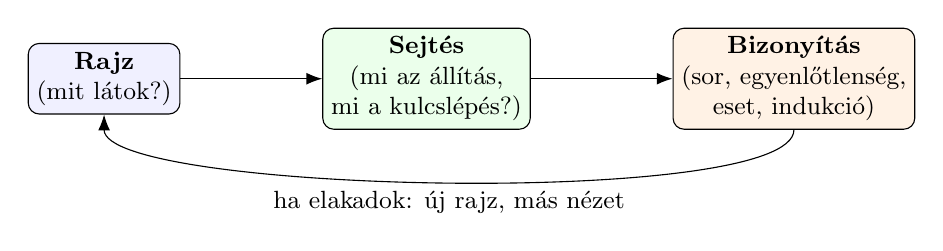
\begin{tikzpicture}[node distance=8mm]
  \node[dob,fill=blue!6] (r) {\textbf{Rajz}\\ (mit látok?)};
  \node[dob,fill=green!8,right=18mm of r] (s) {\textbf{Sejtés}\\ (mi az állítás,\\ mi a kulcslépés?)};
  \node[dob,fill=orange!10,right=18mm of s] (b) {\textbf{Bizonyítás}\\ (sor, egyenlőtlenség,\\ eset, indukció)};
  \draw[nyil] (r) -- (s);
  \draw[nyil] (s) -- (b);
  \draw[nyil] (b.south) .. controls +(0,-10mm) and +(0,-10mm) .. node[below,font=\small]{ha elakadok: új rajz, más nézet} (r.south);
\end{tikzpicture}
\end{center}

\noindent\textbf{Három tipikus rajzhiba.}
\begin{enumerate}[nosep,leftmargin=*]
  \item \emph{Túl szép eset.} Az ábrán a függvény sima és monoton, holott a feladat
        ezt nem mondja (3.14, 4.13). Ellenszer: rajzoljunk szándékosan csúnya ellenpéldát is.
  \item \emph{Elhagyott perempont.} A rajz nem mutatja, hogy az intervallum vége nyitott-e
        (1.4 b, 2.1, 4.9). Ellenszer: üres és tömör karika következetes használata.
  \item \emph{Végtelen mint pont.} A $+\infty$-t helynek rajzoljuk. Ellenszer: a végtelenben
        vett határértéket mindig \emph{sávval} rajzoljuk (\ref{fig:dominans}. ábra).
\end{enumerate}

\section{Logikai rajzok}

\subsection{Venn- és Euler-diagram (1.1, 1.3, 1.4, 1.7, 1.12)}

A Venn-diagram akkor jó, ha \emph{halmazműveletről} vagy \emph{implikációról} van szó:
az $A \subseteq B$ tartalmazás képe a „belül van” reláció, a metszet és unió a szokásos
átfedés. A számhalmazoknál (1.3) inkább Euler-diagramot rajzolunk: egymásba skatulyázott
ovális alakzatokat.

\begin{center}
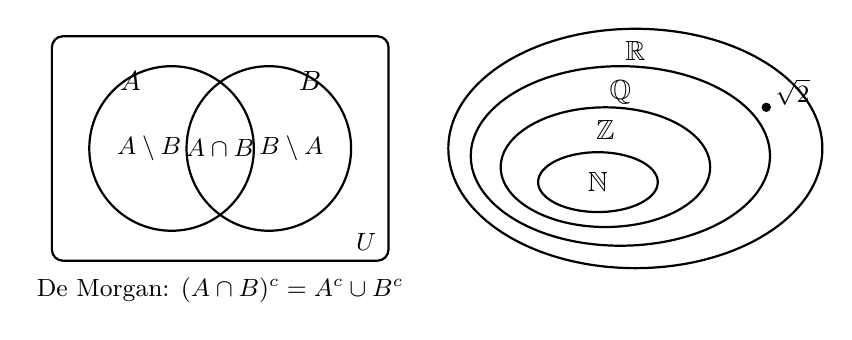
\begin{tikzpicture}[scale=0.95]
  % Venn
  \begin{scope}
    \draw[hal] (0,0) circle (1.1);
    \draw[hal] (1.3,0) circle (1.1);
    \node at (-0.55,0.9) {$A$}; \node at (1.85,0.9) {$B$};
    \node at (-0.3,0) {\small $A\setminus B$};
    \node at (0.65,0) {\small $A\cap B$};
    \node at (1.6,0) {\small $B\setminus A$};
    \draw[hal,rounded corners] (-1.6,-1.5) rectangle (2.9,1.5);
    \node at (2.6,-1.25) {\small $U$};
    \node at (0.65,-1.9) {\small De Morgan: $(A\cap B)^c=A^c\cup B^c$};
  \end{scope}
  % Euler
  \begin{scope}[xshift=6.2cm]
    \draw[hal] (0,0) ellipse (2.5 and 1.6); \node at (0,1.3) {$\R$};
    \draw[hal] (-0.2,-0.1) ellipse (2.0 and 1.2); \node at (-0.2,0.75) {$\Q$};
    \draw[hal] (-0.4,-0.25) ellipse (1.4 and 0.8); \node at (-0.4,0.25) {$\Z$};
    \draw[hal] (-0.5,-0.45) ellipse (0.8 and 0.4); \node at (-0.5,-0.45) {$\N$};
    \node[pont] at (1.75,0.55) {}; \node at (2.1,0.75) {\small $\sqrt2$};
  \end{scope}
\end{tikzpicture}
\end{center}

\begin{fogas}
Az 1.7 a) „a néggyel oszthatók párosak” állítás rajza két egymásba írt kör; a bizonyítás
pedig pontosan az, amit a rajz sugall: \emph{veszünk egy pontot a belső körből}
($n=4k$) és megmutatjuk, hogy a külsőben van ($n=2\cdot 2k$).
Lean-ben ez a \lean{intro n hn} lépés: a rajzbeli „veszünk egy pontot” a
\lean{intro}-nak felel meg.
\end{fogas}

\subsection{A kvantorok játékfája (3.1, 3.14, 4.13)}

Az $\forall \eps>0\ \exists \delta>0\ \forall x\,(\dots)$ állítást olvassuk
\emph{kétszemélyes játéknak}: az Ellenfél választ $\eps$-t, mi választunk $\delta$-t,
majd az Ellenfél választ $x$-et. Az állítás igaz $\iff$ van nyerő stratégiánk, azaz
egy $\delta = D(\eps)$ \emph{függvény}. Ez a rajz teszi nyilvánvalóvá, hogy $\delta$
függhet $\eps$-tól (és a pont helyétől), de $x$-től nem.

\begin{center}
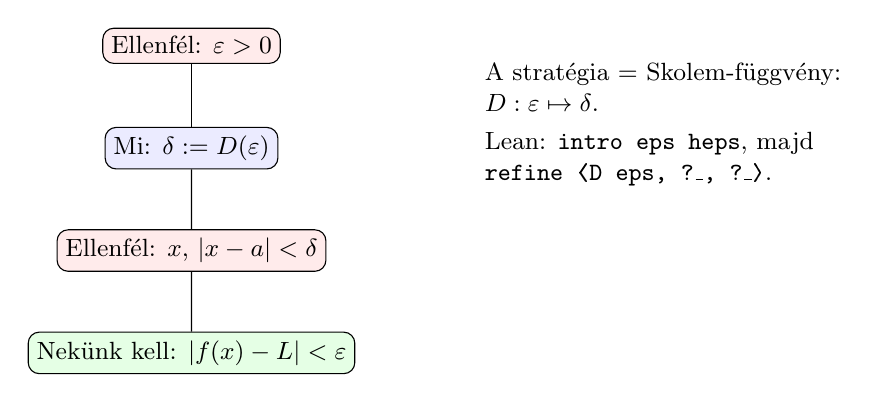
\begin{tikzpicture}[level distance=13mm,
  level 1/.style={sibling distance=34mm},
  level 2/.style={sibling distance=34mm},
  level 3/.style={sibling distance=17mm},font=\small]
  \node[dob,fill=red!8] {Ellenfél: $\eps>0$}
    child {node[dob,fill=blue!8] {Mi: $\delta:=D(\eps)$}
      child {node[dob,fill=red!8] {Ellenfél: $x$, $|x-a|<\delta$}
        child {node[dob,fill=green!10] {Nekünk kell: $|f(x)-L|<\eps$}}}};
  \node[align=left,font=\small,anchor=west] at (3.6,-1.0)
    {A stratégia = Skolem-függvény:\\ $D:\eps \mapsto \delta$.\\[1mm]
     Lean: \lean{intro eps heps}, majd\\ \lean{refine ⟨D eps, ?\_, ?\_⟩}.};
\end{tikzpicture}
\end{center}

A 3.1 a) feladatnál ($\lim_{x\to1}\frac{1}{x^3+2}=\frac13$) a stratégia megkeresése
maga is rajzos: a célsávból ($y$-tengely) visszaolvassuk a megengedett $x$-sávot.

\subsection{Szemantikus tabló: az esetszétválasztás fája (1.12, 3.5, 3.11)}

A tabló-fa egyetlen szabályt használ: \emph{bontsuk a formulát, és ahol „vagy” áll,
ágazzunk el}; egy ág lezárul ($\otimes$), ha ellentmondó feltételek gyűltek össze rajta.
Ez pontosan az abszolút értékes és törtes egyenlőtlenségek megoldásának a váza.

\begin{center}
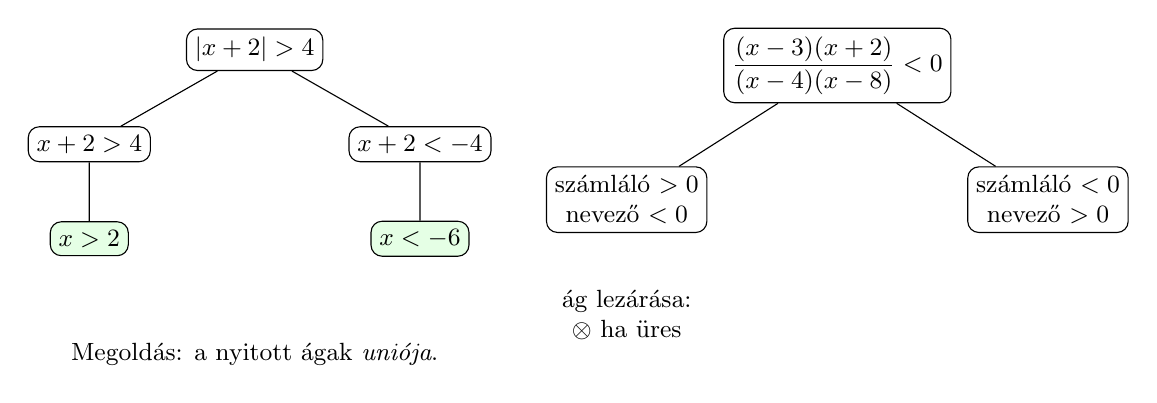
\begin{tikzpicture}[level distance=12mm,
  level 1/.style={sibling distance=42mm},
  level 2/.style={sibling distance=22mm},font=\small]
  \node[dob] {$|x+2|>4$}
    child {node[dob] {$x+2>4$}
      child {node[dob,fill=green!10] {$x>2$}}}
    child {node[dob] {$x+2<-4$}
      child {node[dob,fill=green!10] {$x<-6$}}};
  \node[font=\small,anchor=north] at (0,-3.6) {Megoldás: a nyitott ágak \emph{uniója}.};
  \begin{scope}[xshift=7.4cm,yshift=-0.2cm]
    \node[dob] (a) {$\dfrac{(x-3)(x+2)}{(x-4)(x-8)}<0$};
    \node[dob,below left=8mm and 2mm of a] (b) {számláló $>0$\\ nevező $<0$};
    \node[dob,below right=8mm and 2mm of a] (c) {számláló $<0$\\ nevező $>0$};
    \draw (a) -- (b); \draw (a) -- (c);
    \node[font=\small,below=6mm of b,align=center] {ág lezárása:\\ $\otimes$ ha üres};
  \end{scope}
\end{tikzpicture}
\end{center}

\begin{fogas}[tablófa törtekre]
Törtnél \emph{soha ne szorozzunk} ismeretlen előjelű nevezővel: vagy két ágra bontunk
(nevező pozitív / negatív), vagy — ami rajzban gyorsabb — mindent egy oldalra rendezünk
és előjelvonalat rajzolunk (\ref{sec:elojel}. szakasz). A tabló és az előjelvonal ugyanaz
a gondolat, csak más nézetben.
\end{fogas}

\subsection{Fitch-doboz: a feltevések élettartama}

A Fitch-stílusú doboz azt rajzolja le, hogy \emph{meddig él} egy feltevés. Ez a
kép egy az egyben megfelel a Lean-beli \lean{intro}/\lean{exact} párnak és a papíron
írt „Tegyük fel, hogy \dots\ Tehát \dots” szerkezetnek.

\begin{center}
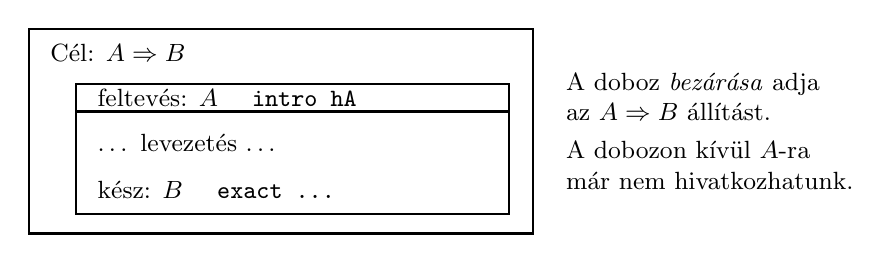
\begin{tikzpicture}[font=\small]
  \draw[thick] (0,0) rectangle (6.4,2.6);
  \node[anchor=west] at (0.15,2.3) {Cél: $A \Rightarrow B$};
  \draw[thick] (0.6,0.25) rectangle (6.1,1.9);
  \draw[thick] (0.6,1.55) -- (6.1,1.55);
  \node[anchor=west] at (0.75,1.72) {feltevés: $A$ \quad \lean{intro hA}};
  \node[anchor=west] at (0.75,1.15) {\dots\ levezetés \dots};
  \node[anchor=west] at (0.75,0.55) {kész: $B$ \quad \lean{exact ...}};
  \node[anchor=west,align=left] at (6.7,1.3)
    {A doboz \emph{bezárása} adja\\ az $A\Rightarrow B$ állítást.\\[1mm]
     A dobozon kívül $A$-ra\\ már nem hivatkozhatunk.};
\end{tikzpicture}
\end{center}

\subsection{Átlós tábla: önhivatkozás (1.2)}

A juhászos feladat (Russell-paradoxon) rajza egy négyzetrács: a sorok és oszlopok
ugyanazok a gazdák, a $(b,a)$ mezőben pipa áll, ha $b$ vigyáz $a$ birkáira.
A „jó falusi juhász” sora definíció szerint az \emph{átló tagadása} — de akkor a saját
átlóbeli mezője önmagával kerül ellentmondásba.

\begin{center}
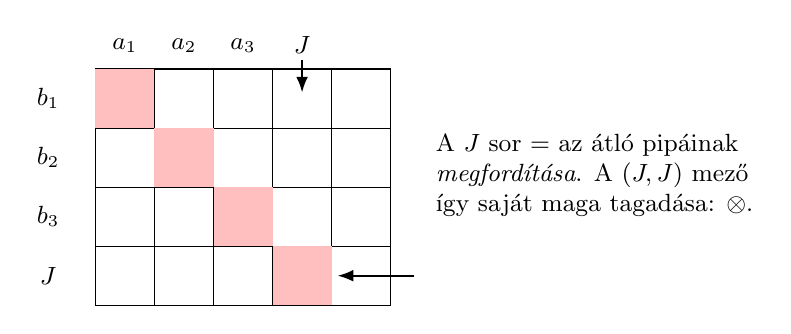
\begin{tikzpicture}[scale=0.75,font=\small]
  \foreach \i in {0,...,4} \draw (0,\i) -- (5,\i);
  \foreach \j in {0,...,5} \draw (\j,0) -- (\j,4);
  \foreach \k in {0,...,3} \fill[red!25] (\k,3-\k) rectangle (\k+1,4-\k);
  \node at (-0.8,3.5) {$b_1$}; \node at (-0.8,2.5) {$b_2$};
  \node at (-0.8,1.5) {$b_3$}; \node at (-0.8,0.5) {$J$};
  \node at (0.5,4.4) {$a_1$}; \node at (1.5,4.4) {$a_2$};
  \node at (2.5,4.4) {$a_3$}; \node at (3.5,4.4) {$J$};
  \node[align=left,anchor=west] at (5.6,2.2)
    {A $J$ sor $=$ az átló pipáinak\\ \emph{megfordítása}. A $(J,J)$ mező\\
     így saját maga tagadása: $\otimes$.};
  \draw[nyil,thick] (5.4,0.5) -- (4.1,0.5);
  \draw[nyil,thick] (3.5,4.15) -- (3.5,3.6);
\end{tikzpicture}
\end{center}

\noindent Pontos tartalom (Lean): \lean{Kalkulus1.Rajzok.atlos\_tabla}, azaz
$\neg\exists b\ \forall a\,\bigl(R(b,a)\leftrightarrow \neg R(a,a)\bigr)$.
Ugyanez a rajz adja Cantor átlós tételét is — érdemes egyszer végigrajzolni.

\subsection{Skatulyák (1.10)}

Az 1.10 a) feladathoz rajzoljunk egy $[0,1)$ szakaszt $n+1$ rekesszel, és tegyük bele a
$0\cdot x,\,1\cdot x,\,\dots,\,n\cdot x$ számok törtrészeit: $n+1$ pont, $n+1$ rekesz,
de a két végpont miatt \emph{két pont ugyanabba a rekeszbe} esik. A különbségük egy
$k x - j$ alakú, kicsi szám — épp a kívánt közelítés.

\begin{center}
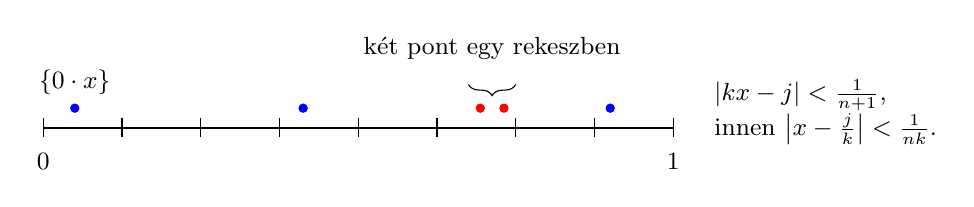
\begin{tikzpicture}[scale=1.0,font=\small]
  \draw[seg] (0,0) -- (8,0);
  \foreach \i in {0,...,8} \draw (\i,-0.12) -- (\i,0.12);
  \node[below] at (0,-0.2) {$0$}; \node[below] at (8,-0.2) {$1$};
  \node[pont,fill=blue] at (0.4,0.25) {}; \node[above] at (0.4,0.3) {$\{0\cdot x\}$};
  \node[pont,fill=blue] at (3.3,0.25) {};
  \node[pont,fill=red] at (5.55,0.25) {}; \node[pont,fill=red] at (5.85,0.25) {};
  \node[pont,fill=blue] at (7.2,0.25) {};
  \draw[decorate,decoration={brace,amplitude=4pt}] (6,0.55) -- (5.4,0.55);
  \node[above] at (5.7,0.75) {két pont egy rekeszben};
  \node[align=left,anchor=west] at (8.4,0.2) {$|kx-j| < \frac{1}{n+1}$,\\ innen $\bigl|x-\frac{j}{k}\bigr| < \frac{1}{nk}$.};
\end{tikzpicture}
\end{center}

\noindent Lean: \lean{Kalkulus1.Rajzok.skatulyaelv\_kozelites}.

\section{Számegyenes-rajzok}

\subsection{Abszolút érték $=$ távolság (1.11, 1.12 h--j, 3.1)}

Az $|u-v|$ kifejezést mindig \emph{távolságnak} olvassuk. Ekkor
$|x-5|\le \eps$ nem egyenlőtlenség, hanem egy \emph{sáv} a számegyenesen, a
háromszög-egyenlőtlenség pedig „kerülővel nem rövidebb az út”.

\begin{center}
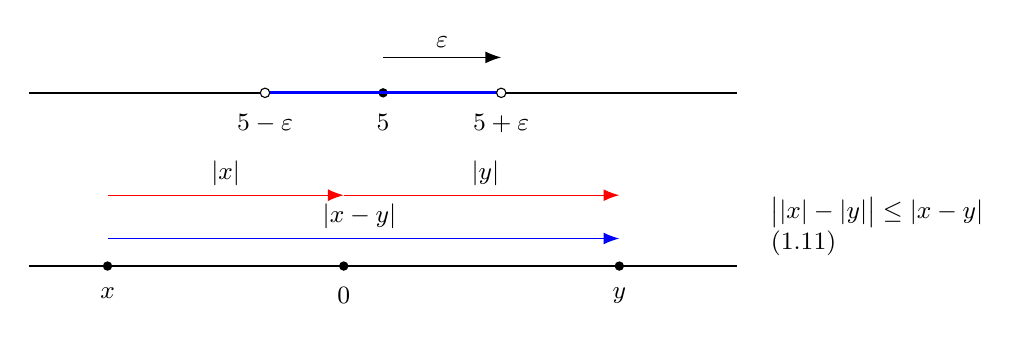
\begin{tikzpicture}[font=\small]
  \draw[seg] (0,0) -- (9,0);
  \node[pont] at (4.5,0) {}; \node[below] at (4.5,-0.15) {$5$};
  \draw[very thick,blue] (3,0) -- (6,0);
  \node[ures] at (3,0) {}; \node[ures] at (6,0) {};
  \node[below] at (3,-0.15) {$5-\eps$}; \node[below] at (6,-0.15) {$5+\eps$};
  \draw[nyil] (4.5,0.45) -- (6,0.45); \node[above] at (5.25,0.45) {$\eps$};
  % triangle inequality
  \begin{scope}[yshift=-2.2cm]
    \draw[seg] (0,0) -- (9,0);
    \node[pont] at (1,0) {}; \node[below] at (1,-0.15) {$x$};
    \node[pont] at (4,0) {}; \node[below] at (4,-0.15) {$0$};
    \node[pont] at (7.5,0) {}; \node[below] at (7.5,-0.15) {$y$};
    \draw[nyil,blue] (1,0.35) -- (7.5,0.35); \node[above] at (4.2,0.35) {$|x-y|$};
    \draw[nyil,red] (1,0.9) -- (4,0.9); \node[above] at (2.5,0.9) {$|x|$};
    \draw[nyil,red] (4,0.9) -- (7.5,0.9); \node[above] at (5.8,0.9) {$|y|$};
    \node[anchor=west,align=left] at (9.3,0.5) {$\bigl||x|-|y|\bigr| \le |x-y|$\\ (1.11)};
  \end{scope}
\end{tikzpicture}
\end{center}

\subsection{Előjelvonal: a legjobb papírtechnika}\label{sec:elojel}

Racionális törtes egyenlőtlenségnél (1.12 c--g), pólusoknál (3.8, 3.9) és
menetvizsgálatnál (4.8) ugyanaz a rajz működik: a nevező és a számláló
\emph{gyökeit és pólusait} felvisszük a számegyenesre, majd tényezőnként
$+/-$ jeleket írunk, és szorozzuk az oszlopokat.

\begin{center}
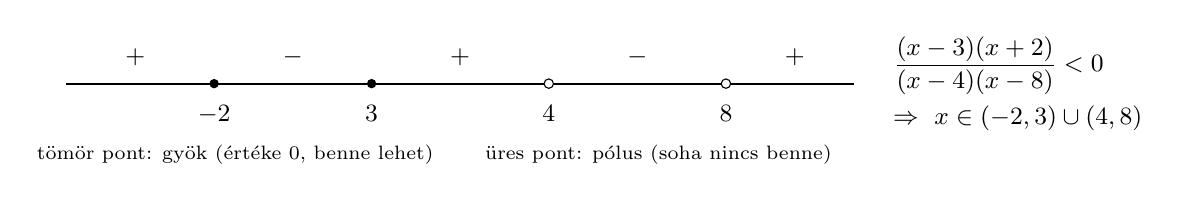
\begin{tikzpicture}[font=\small,xscale=1.25]
  \draw[seg] (-0.5,0) -- (7.5,0);
  \foreach \x/\lab in {1/{-2}, 2.6/3} {
    \node[pont] at (\x,0) {};
    \node[below] at (\x,-0.15) {$\lab$};
  }
  \foreach \x/\lab in {4.4/4, 6.2/8} {
    \node[ures] at (\x,0) {};
    \node[below] at (\x,-0.15) {$\lab$};
  }
  \node[above,align=center] at (0.2,0.1) {$+$};
  \node[above,align=center] at (1.8,0.1) {$-$};
  \node[above,align=center] at (3.5,0.1) {$+$};
  \node[above,align=center] at (5.3,0.1) {$-$};
  \node[above,align=center] at (6.9,0.1) {$+$};
  \node[anchor=west,align=left] at (7.8,0)
    {$\dfrac{(x-3)(x+2)}{(x-4)(x-8)}<0$\\[1mm]
     $\Rightarrow\ x\in(-2,3)\cup(4,8)$};
  \node[anchor=west,align=left,font=\scriptsize] at (-0.9,-0.9)
    {tömör pont: gyök (értéke $0$, benne lehet) \qquad üres pont: pólus (soha nincs benne)};
\end{tikzpicture}
\end{center}

\noindent A rajz \emph{miért} működik: két gyöktényező szorzata pontosan a gyökök között
negatív; pontos alak Leanben: \lean{Kalkulus1.Rajzok.elojel\_vonal}.

\subsection{Gátak: felső/alsó határ (1.4, 1.5, 3.14)}

A korlát „fal” a számegyenesen; a szuprémum a \emph{legbaloldalibb} fal. Ebből a képből
azonnal látszik a szuprémum két tulajdonsága (felső korlát; minden nála kisebb szám már
nem az), és az egyértelműség is: két legbaloldalibb fal csak egybeeshet.

\begin{center}
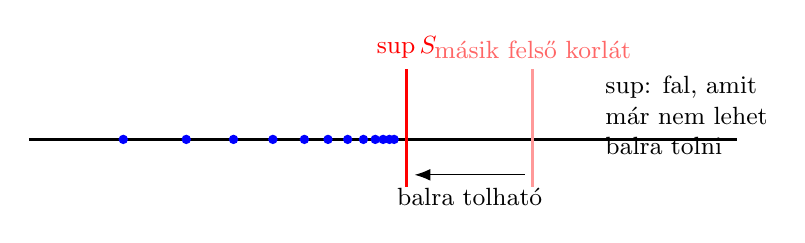
\begin{tikzpicture}[font=\small]
  \draw[seg] (0,0) -- (9,0);
  \foreach \x in {1.2,2.0,2.6,3.1,3.5,3.8,4.05,4.25,4.4,4.5,4.58,4.64}
     \node[pont,blue] at (\x,0) {};
  \draw[very thick,red] (4.8,-0.6) -- (4.8,0.9);
  \node[red,above] at (4.8,0.9) {$\sup S$};
  \draw[very thick,red!40] (6.4,-0.6) -- (6.4,0.9);
  \node[red!60,above] at (6.4,0.9) {másik felső korlát};
  \draw[nyil] (6.3,-0.45) -- (4.9,-0.45);
  \node[below] at (5.6,-0.5) {balra tolható};
  \node[anchor=west,align=left] at (7.2,0.3)
    {$\sup$: fal, amit\\ már nem lehet\\ balra tolni};
\end{tikzpicture}
\end{center}

\subsection{Nagyítás és felezés (1.6, 3.15, 4.13)}

A béka-feladat (1.6) rajza: a $[0,1]$ szakaszt mindig félbevágjuk; a részletösszeg
$1-2^{-n}$, a maradék a jobb oldali kis szakasz. Ugyanez a felezéses rajz tér vissza a
középponti konvexitásnál (4.13) és a diadikus racionálisoknál (3.15).

\begin{center}
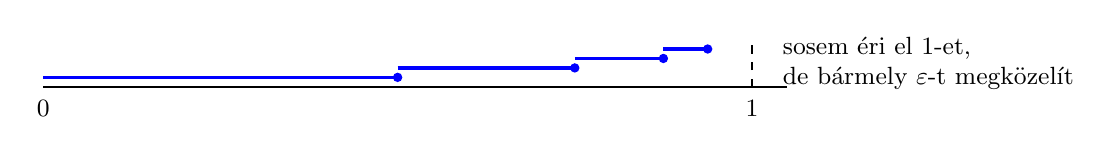
\begin{tikzpicture}[font=\small,xscale=9,yscale=1]
  \draw[seg] (0,0) -- (1.05,0);
  \node[below] at (0,-0.05) {$0$}; \node[below] at (1,-0.05) {$1$};
  \foreach \n/\a/\b in {1/0/0.5, 2/0.5/0.75, 3/0.75/0.875, 4/0.875/0.9375} {
    \draw[very thick,blue] (\a,0.12*\n) -- (\b,0.12*\n);
    \node[pont,blue] at (\b,0.12*\n) {};
  }
  \draw[dashed] (1,0) -- (1,0.55);
  \node[anchor=west,align=left] at (1.03,0.3) {sosem éri el $1$-et,\\ de bármely $\eps$-t megközelít};
\end{tikzpicture}
\end{center}

\subsection{Négyzetrajz a $\sqrt2$ irracionalitásához (1.9)}

A klasszikus paritásos bizonyítás mellett érdemes a Tennenbaum-féle képet is ismerni:
ha $\sqrt2=p/q$ a legkisebb ilyen nevezővel, akkor két $q\times q$-s négyzet együtt épp
egy $p\times p$-s négyzetet ad ki; a középső átfedés és a két kimaradó sarok viszont
\emph{kisebb} nevezőjű megoldást szolgáltat --- ellentmondás.

\begin{center}
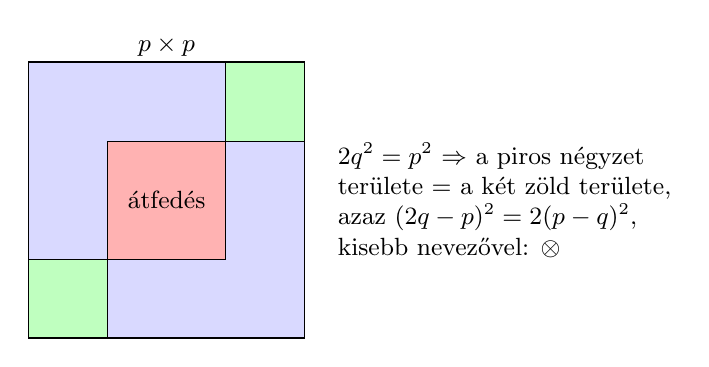
\begin{tikzpicture}[scale=0.5,font=\small]
  \draw[hal] (0,0) rectangle (7,7); \node at (3.5,7.4) {$p\times p$};
  \draw[fill=blue!15] (0,2) rectangle (5,7);
  \draw[fill=blue!15] (2,0) rectangle (7,5);
  \draw[fill=red!30] (2,2) rectangle (5,5);
  \node at (3.5,3.5) {\small átfedés};
  \draw[fill=green!25] (0,0) rectangle (2,2);
  \draw[fill=green!25] (5,5) rectangle (7,7);
  \node[anchor=west,align=left] at (7.6,3.5)
    {$2q^2=p^2$ $\Rightarrow$ a piros négyzet\\ területe $=$ a két zöld területe,\\
     azaz $(2q-p)^2=2(p-q)^2$,\\ kisebb nevezővel: $\otimes$};
\end{tikzpicture}
\end{center}

\section{Indukció és véges összegek: kirakós rajzok}

\subsection{Dominó (minden indukció)}

Az indukció rajza két dolog: az \emph{első} dominó eldől (bázis), és \emph{bármelyik}
eldőlő dominó eldönti a következőt (lépés). A gyakorlatban a lépés rajza a fontos:
mit teszünk hozzá az $n$-edikről az $(n+1)$-edikre.

\begin{center}
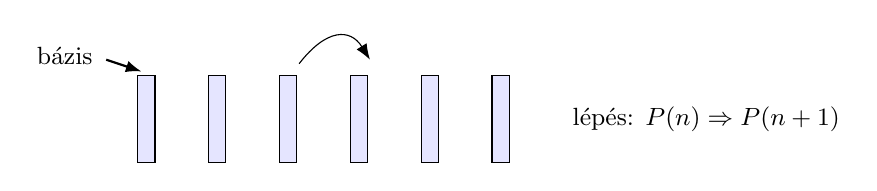
\begin{tikzpicture}[font=\small]
  \foreach \i in {0,...,5} {
    \draw[fill=blue!10] (\i*0.9,0) rectangle (\i*0.9+0.22,1.1);
  }
  \draw[nyil,thick] (-0.4,1.3) -- (0.05,1.15);
  \node[anchor=east] at (-0.45,1.35) {bázis};
  \node[anchor=west,align=left] at (5.4,0.55) {lépés: $P(n)\Rightarrow P(n+1)$};
  \draw[nyil] (2.05,1.25) .. controls (2.4,1.7) and (2.7,1.7) .. (2.95,1.3);
\end{tikzpicture}
\end{center}

\subsection{Gauss-téglalap (1.14 a) és a négyzetszámok (1.16)}

Az $1+2+\dots+n$ lépcsőt megduplázva és elforgatva $n\times(n+1)$-es téglalapot kapunk.
Ugyanez a trükk működik a négyzetszámokra: három lépcsőtorony egy
$(2n+1)$ magas hasábbá rendezhető, ami épp a
$3\sum i^2=(2n+1)\sum i$ azonosság --- innen a zárt alak \emph{indukció nélkül} jön.

\begin{center}
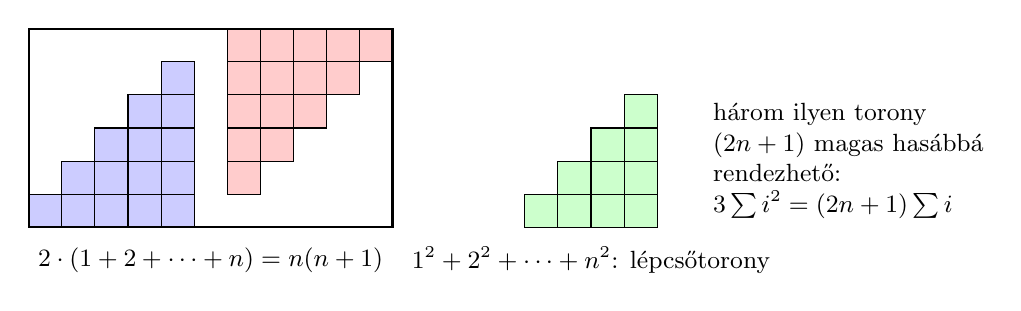
\begin{tikzpicture}[scale=0.42,font=\small]
  \foreach \i in {1,...,5} \foreach \j in {1,...,\i}
     \draw[fill=blue!20] (\i-1,\j-1) rectangle (\i,\j);
  \foreach \i in {1,...,5} \foreach \j in {1,...,\i}
     \draw[fill=red!20] (11-\i,6-\j) rectangle (12-\i,7-\j);
  \draw[thick] (0,0) rectangle (11,6);
  \node at (5.5,-1) {$2\cdot(1+2+\dots+n) = n(n+1)$};
  \begin{scope}[xshift=15cm]
    \foreach \i in {1,...,4} \foreach \j in {1,...,\i}
      \draw[fill=green!20] (\i-1,\j-1) rectangle (\i,\j);
    \node at (2,-1) {$1^2+2^2+\dots+n^2$: lépcsőtorony};
    \node[anchor=west,align=left] at (5.4,2)
      {három ilyen torony\\ $(2n+1)$ magas hasábbá\\ rendezhető:\\
       $3\sum i^2=(2n+1)\sum i$};
  \end{scope}
\end{tikzpicture}
\end{center}

\noindent Lean: \lean{Kalkulus1.Rajzok.negyzetszamok\_kepe} és
\lean{Kalkulus1.Rajzok.gauss\_teglalap}.

\subsection{Teleszkópos téglalapok (1.15 c, 1.17)}\label{sec:teleszkop}

A $\sum 1/\sqrt i$ becslésénél a rajz: az $1/\sqrt x$ görbe alatti terület téglalapokkal
közrefogva. A papíron használt algebrai megfelelője a
$\frac{1}{\sqrt i} < 2(\sqrt i-\sqrt{i-1})$ becslés, amit összegezve minden belső tag kiesik.

\begin{center}
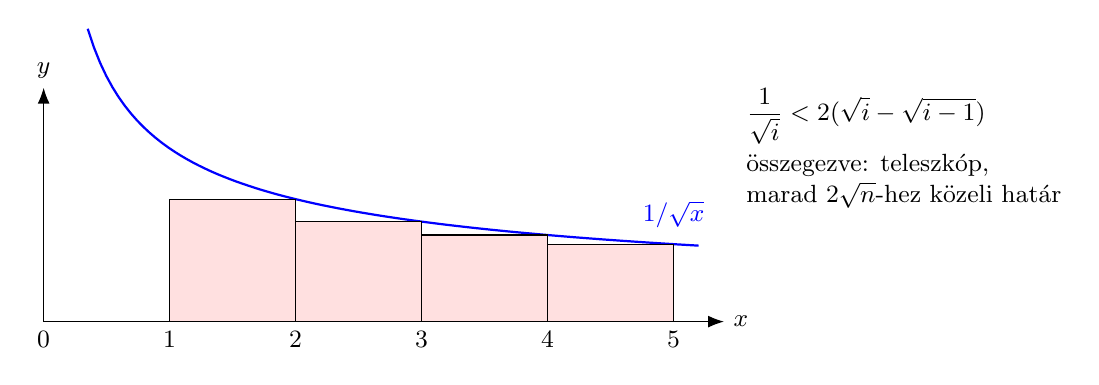
\begin{tikzpicture}[font=\small,xscale=1.6,yscale=2.2]
  \draw[nyil] (0,0) -- (5.4,0) node[right] {$x$};
  \draw[nyil] (0,0) -- (0,1.35) node[above] {$y$};
  \draw[domain=0.35:5.2,samples=100,thick,blue] plot (\x, {1/sqrt(\x)});
  \node[blue] at (5.0,0.62) {$1/\sqrt x$};
  \foreach \i in {1,...,4} {
    \draw[fill=red!12] (\i,0) rectangle (\i+1, {1/sqrt(\i+1)});
  }
  \foreach \i in {0,...,5} \node[below] at (\i,0) {$\i$};
  \node[anchor=west,align=left] at (5.5,1.0)
    {$\displaystyle\frac{1}{\sqrt i} < 2(\sqrt i - \sqrt{i-1})$\\[1mm]
     összegezve: teleszkóp,\\ marad $2\sqrt n$-hez közeli határ};
\end{tikzpicture}
\end{center}

\subsection{Pascal-háromszög mint rácsutak (1.19)}

A $\binom{n}{k}$ szám a rácson vezető, jobbra/felfelé lépő utak száma. Ekkor
\begin{itemize}[nosep]
  \item 1.19 a) az utolsó lépés két lehetősége: $\binom{n-1}{k-1}+\binom{n-1}{k}=\binom{n}{k}$;
  \item 1.19 b) a binomiális tétel: $n$ dobozból választunk $k$-t, ahol $b$-t viszünk;
  \item 1.19 c) a „hokiütő”: az utakat aszerint osztályozzuk, hol lépünk utoljára felfelé.
\end{itemize}

\begin{center}
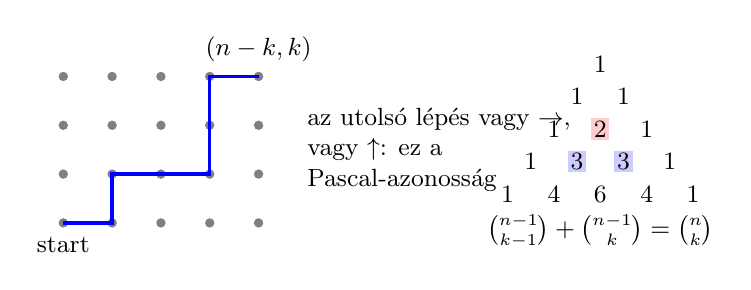
\begin{tikzpicture}[scale=0.62,font=\small]
  \foreach \i in {0,...,4} \foreach \j in {0,...,3} \node[pont,gray] at (\i,\j) {};
  \draw[very thick,blue] (0,0) -- (1,0) -- (1,1) -- (3,1) -- (3,3) -- (4,3);
  \node[below] at (0,-0.1) {start}; \node[above] at (4,3.1) {$(n-k,k)$};
  \node[anchor=west,align=left] at (4.8,1.5)
    {az utolsó lépés vagy $\rightarrow$,\\ vagy $\uparrow$: ez a\\ Pascal-azonosság};
  \begin{scope}[xshift=11cm,yshift=0.4cm,scale=0.95]
    \node at (0,3) {$1$};
    \node at (-0.5,2.3) {$1$}; \node at (0.5,2.3) {$1$};
    \node at (-1,1.6) {$1$}; \node[fill=red!20,inner sep=1pt] at (0,1.6) {$2$}; \node at (1,1.6) {$1$};
    \node at (-1.5,0.9) {$1$}; \node[fill=blue!20,inner sep=1pt] at (-0.5,0.9) {$3$};
    \node[fill=blue!20,inner sep=1pt] at (0.5,0.9) {$3$}; \node at (1.5,0.9) {$1$};
    \node at (-2,0.2) {$1$}; \node at (-1,0.2) {$4$}; \node at (0,0.2) {$6$};
    \node at (1,0.2) {$4$}; \node at (2,0.2) {$1$};
    \node at (0,-0.6) {$\binom{n-1}{k-1}+\binom{n-1}{k}=\binom{n}{k}$};
  \end{scope}
\end{tikzpicture}
\end{center}

\subsection{Párosítás: $n! < \bigl(\frac{n+1}{2}\bigr)^n$ (1.15 d)}

A rajz: írjuk föl a szorzatot kétszer, egyszer növekvő, egyszer csökkenő sorrendben, és
párosítsuk az egymás alá kerülő tagokat. Minden párra $i(n+1-i) \le \left(\frac{n+1}{2}\right)^2$
(számtani--mértani közép, azaz „adott kerületű téglalapok közül a négyzet a legnagyobb területű”).

\begin{center}
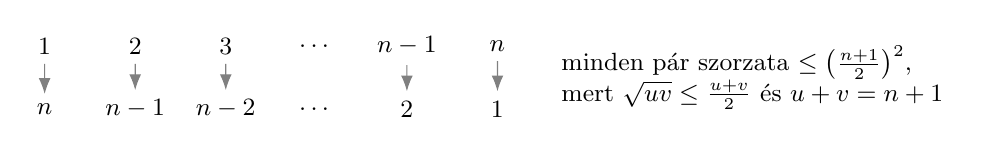
\begin{tikzpicture}[font=\small,xscale=1.15]
  \foreach \i/\lab in {1/1,2/2,3/3,4/{\dots},5/{n-1},6/n}
    \node (a\i) at (\i,0.8) {$\lab$};
  \foreach \i/\lab in {1/n,2/{n-1},3/{n-2},4/{\dots},5/2,6/1}
    \node (b\i) at (\i,0) {$\lab$};
  \foreach \i in {1,2,3,5,6} \draw[nyil,gray] (a\i) -- (b\i);
  \node[anchor=west,align=left] at (6.6,0.4)
    {minden pár szorzata $\le \left(\frac{n+1}{2}\right)^2$,\\
     mert $\sqrt{uv}\le \frac{u+v}{2}$ és $u+v=n+1$};
\end{tikzpicture}
\end{center}

\section{Függvények: koordinátarendszer-rajzok}

\subsection{Értelmezési tartomány mint szűrők metszete (2.1)}

Minden „veszélyes” művelet egy-egy \emph{feltételt} tesz a számegyenesre:
gyök alatt $\ge 0$, nevezőben $\ne 0$, logaritmusban $>0$, $\arccos$-ban $[-1,1]$.
Rajzoljuk mindegyiket külön sávként egymás alá, és a válasz a sávok metszete.

\begin{center}
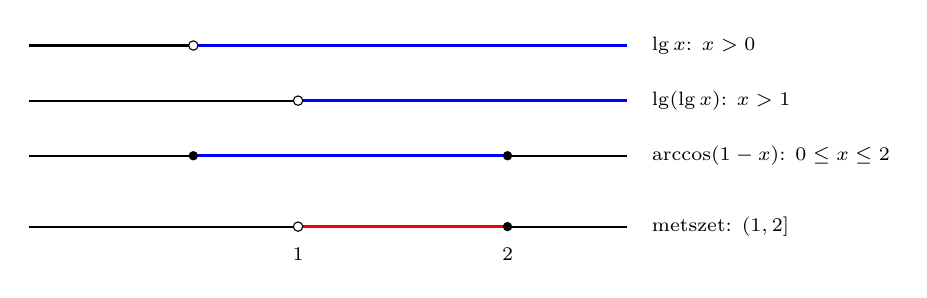
\begin{tikzpicture}[font=\small,xscale=0.95]
  \foreach \y/\lab in {0/{$\lg x$: $x>0$}, -0.7/{$\lg(\lg x)$: $x>1$}, -1.4/{$\arccos(1-x)$: $0\le x\le 2$}} {
    \draw[seg] (0,\y) -- (8,\y);
    \node[anchor=west,font=\scriptsize] at (8.2,\y) {\lab};
  }
  \draw[very thick,blue] (2.2,0) -- (8,0); \node[ures] at (2.2,0) {};
  \draw[very thick,blue] (3.6,-0.7) -- (8,-0.7); \node[ures] at (3.6,-0.7) {};
  \draw[very thick,blue] (2.2,-1.4) -- (6.4,-1.4);
  \node[pont] at (2.2,-1.4) {}; \node[pont] at (6.4,-1.4) {};
  \draw[seg] (0,-2.3) -- (8,-2.3);
  \draw[very thick,red] (3.6,-2.3) -- (6.4,-2.3);
  \node[ures] at (3.6,-2.3) {}; \node[pont] at (6.4,-2.3) {};
  \node[anchor=west,font=\scriptsize] at (8.2,-2.3) {metszet: $(1,2]$};
  \node[below,font=\scriptsize] at (3.6,-2.45) {$1$};
  \node[below,font=\scriptsize] at (6.4,-2.45) {$2$};
\end{tikzpicture}
\end{center}

\subsection{Vonaltesztek: injektív, szürjektív, bijektív (2.2, 2.6)}

\begin{center}
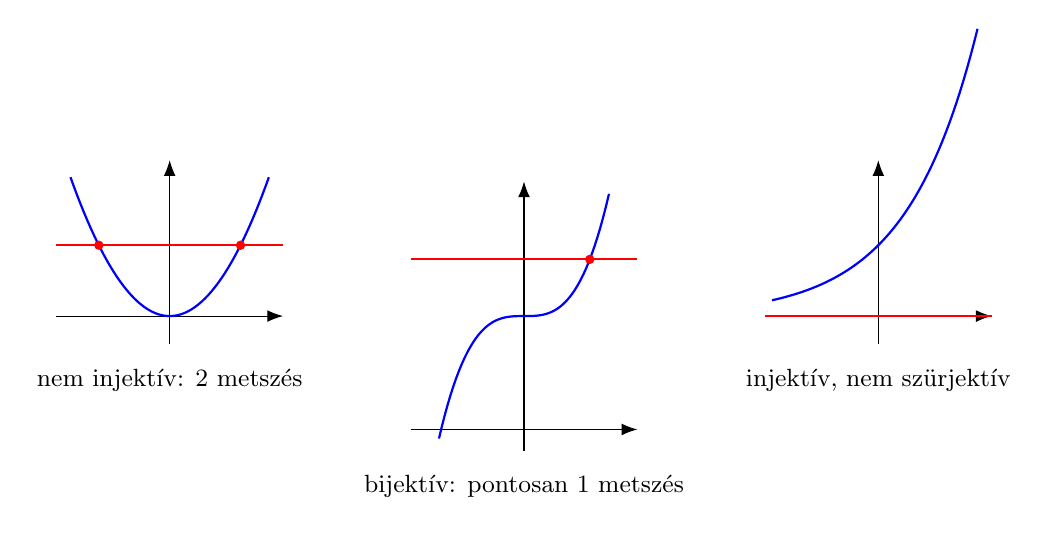
\begin{tikzpicture}[font=\small,scale=0.9]
  \begin{scope}
    \draw[nyil] (-1.6,0) -- (1.6,0); \draw[nyil] (0,-0.4) -- (0,2.2);
    \draw[domain=-1.4:1.4,samples=60,thick,blue] plot (\x,{\x*\x});
    \draw[red,thick] (-1.6,1) -- (1.6,1);
    \node[pont,red] at (-1,1) {}; \node[pont,red] at (1,1) {};
    \node at (0,-0.9) {nem injektív: $2$ metszés};
  \end{scope}
  \begin{scope}[xshift=5cm]
    \draw[nyil] (-1.6,-1.6) -- (1.6,-1.6) ; \draw[nyil] (0,-1.9) -- (0,1.9);
    \draw[domain=-1.2:1.2,samples=60,thick,blue] plot (\x,{\x*\x*\x});
    \draw[red,thick] (-1.6,0.8) -- (1.6,0.8);
    \node[pont,red] at (0.928,0.8) {};
    \node at (0,-2.4) {bijektív: pontosan $1$ metszés};
  \end{scope}
  \begin{scope}[xshift=10cm]
    \draw[nyil] (-1.6,0) -- (1.6,0); \draw[nyil] (0,-0.4) -- (0,2.2);
    \draw[domain=-1.5:1.4,samples=60,thick,blue] plot (\x,{exp(\x)});
    \draw[red,thick] (-1.6,-0.0) -- (1.6,0.0);
    \node at (0,-0.9) {injektív, nem szürjektív};
  \end{scope}
\end{tikzpicture}
\end{center}

\noindent Lean: \lean{Kalkulus1.Rajzok.vizszintes\_vonal\_teszt} és
\lean{szurjektiv\_vonal\_teszt} — a rajz szó szerinti átirata.
Fontos, hogy a teszt csak akkor dönt, ha a \emph{teljes} értelmezési tartományt látjuk:
a 2.2 a) feladatban $a:[0,1]\to[0,1]$, $a(x)=x^2$ már injektív, mert a bal ága hiányzik.

\subsection{Inverz $=$ tükrözés az $y=x$ egyenesre (2.3--2.9)}

\begin{center}
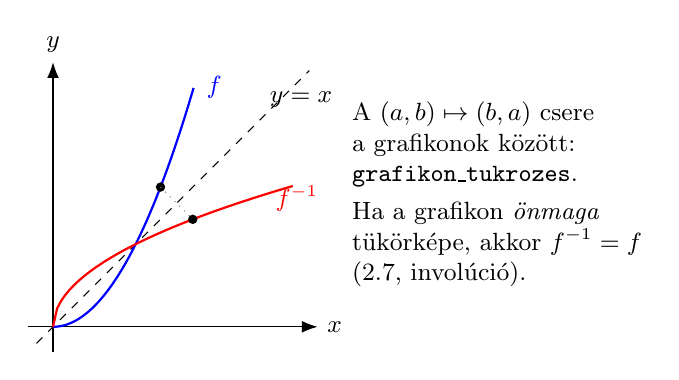
\begin{tikzpicture}[font=\small,scale=1.05]
  \draw[nyil] (-0.3,0) -- (3.2,0) node[right] {$x$};
  \draw[nyil] (0,-0.3) -- (0,3.2) node[above] {$y$};
  \draw[dashed] (-0.2,-0.2) -- (3.1,3.1); \node at (3.0,2.75) {$y=x$};
  \draw[domain=0:1.7,samples=60,thick,blue] plot (\x,{\x*\x});
  \node[blue] at (1.95,2.9) {$f$};
  \draw[domain=0:2.9,samples=60,thick,red] plot (\x,{sqrt(\x)});
  \node[red] at (2.95,1.55) {$f^{-1}$};
  \node[pont] at (1.3,1.69) {}; \node[pont] at (1.69,1.3) {};
  \draw[gray,dotted] (1.3,1.69) -- (1.69,1.3);
  \node[anchor=west,align=left] at (3.5,1.6)
    {A $(a,b)\mapsto(b,a)$ csere\\ a grafikonok között:\\
     \lean{grafikon\_tukrozes}.\\[1mm]
     Ha a grafikon \emph{önmaga}\\ tükörképe, akkor $f^{-1}=f$\\ (2.7, involúció).};
\end{tikzpicture}
\end{center}

\begin{fogas}[2.5, 2.9 típusú feladatok]
Ha a függvény nem injektív, a rajz megmutatja, hol kell \emph{elvágni}: a parabola
csúcsánál, a $\tan$ periódusainál. Az inverz képlete ezután automatikus: cseréljük fel
$x$-et és $y$-t, és oldjuk meg $y$-ra --- ez ugyanaz, mint a tükrözés.
\end{fogas}

\subsection{Kompozíció: átvezető diagram és kommutatív háromszög (2.10--2.15)}

Kompozíciónál két rajz működik együtt: a \emph{halmazszintű} nyíldiagram (mi hova megy)
és a \emph{kétlépcsős} grafikonos átvezetés (a belső függvény értéke lesz a külső bemenete).

\begin{center}
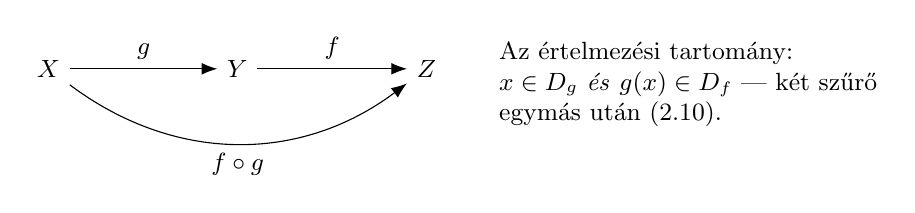
\begin{tikzpicture}[font=\small]
  \node (X) at (0,0) {$X$}; \node (Y) at (2.4,0) {$Y$}; \node (Z) at (4.8,0) {$Z$};
  \draw[nyil] (X) -- node[above] {$g$} (Y);
  \draw[nyil] (Y) -- node[above] {$f$} (Z);
  \draw[nyil] (X) .. controls (1.6,-1.2) and (3.2,-1.2) .. node[below] {$f\circ g$} (Z);
  \node[anchor=west,align=left] at (5.6,-0.2)
    {Az értelmezési tartomány:\\ $x\in D_g$ \emph{és} $g(x)\in D_f$ --- két szűrő\\
     egymás után (2.10).};
\end{tikzpicture}
\end{center}

\noindent A 2.11 feladat ($f(x)=2x^2-1$, $g(x)=4x^3-3x$, $f\circ g=g\circ f$) mögött a
$x=\cos t$ helyettesítés rajza áll: $f(\cos t)=\cos 2t$, $g(\cos t)=\cos 3t$, és
$\cos 2(3t)=\cos 3(2t)$ --- a kommutáló négyzet a szorzás kommutativitása.

\begin{center}
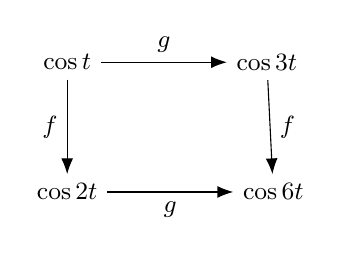
\begin{tikzpicture}[font=\small,node distance=16mm]
  \node (a) {$\cos t$};
  \node (b) [right=of a] {$\cos 3t$};
  \node (c) [below=12mm of a] {$\cos 2t$};
  \node (d) [right=of c] {$\cos 6t$};
  \draw[nyil] (a) -- node[above] {$g$} (b);
  \draw[nyil] (a) -- node[left] {$f$} (c);
  \draw[nyil] (b) -- node[right] {$f$} (d);
  \draw[nyil] (c) -- node[below] {$g$} (d);
\end{tikzpicture}
\end{center}

\subsection{Transzformációk sorrendje (2.16)}

A $-2(x+1)^2+4$ típusú képleteket „recept-fának” rajzoljuk: belülről kifelé haladunk,
és minden lépéshez tartozik egy mozdulat a rajzon.

\begin{center}
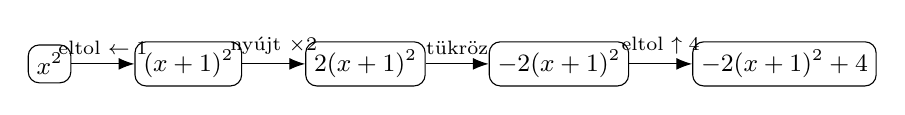
\begin{tikzpicture}[font=\small,node distance=6mm]
  \node[dob] (1) {$x^2$};
  \node[dob,right=8mm of 1] (2) {$(x+1)^2$};
  \node[dob,right=8mm of 2] (3) {$2(x+1)^2$};
  \node[dob,right=8mm of 3] (4) {$-2(x+1)^2$};
  \node[dob,right=8mm of 4] (5) {$-2(x+1)^2+4$};
  \draw[nyil] (1) -- node[above,font=\scriptsize] {eltol $\leftarrow 1$} (2);
  \draw[nyil] (2) -- node[above,font=\scriptsize] {nyújt $\times2$} (3);
  \draw[nyil] (3) -- node[above,font=\scriptsize] {tükröz} (4);
  \draw[nyil] (4) -- node[above,font=\scriptsize] {eltol $\uparrow 4$} (5);
\end{tikzpicture}
\end{center}

\noindent Vigyázat: a \emph{vízszintes} lépések fordítva viselkednek ($x+1$ balra tol),
a függőlegesek természetesen. Ez a leggyakoribb hibaforrás; a rajzon egy kontrollpont
(pl.\ a csúcs) végigkövetése azonnal ellenőrzi.

\subsection{Polinom gyökei és előjelváltás (2.19, 2.20)}

A 2.19 feladat rajza: minden gyöknél kiemelhető egy $(x-c)$ tényező, és a fokszám
eggyel csökken --- a rajz egy „lefelé haladó lépcső”. A 2.20-hoz a gyöktényezős alak
előjelrajza kell: páros multiplicitásnál a grafikon \emph{érinti}, páratlannál
\emph{átmetszi} a tengelyt.

\begin{center}
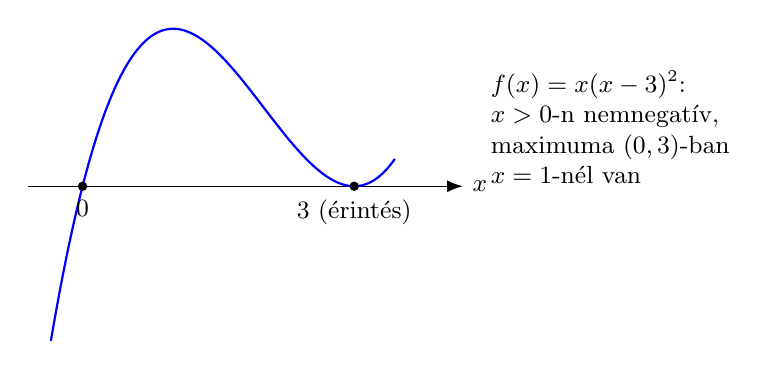
\begin{tikzpicture}[font=\small,xscale=1.15,yscale=0.5]
  \draw[nyil] (-0.6,0) -- (4.2,0) node[right] {$x$};
  \draw[domain=-0.35:3.45,samples=120,thick,blue] plot (\x,{\x*(\x-3)*(\x-3)});
  \node[pont] at (0,0) {}; \node[below] at (0,-0.1) {$0$};
  \node[pont] at (3,0) {}; \node[below] at (3,-0.1) {$3$ (érintés)};
  \node[anchor=west,align=left] at (4.4,1.5)
    {$f(x)=x(x-3)^2$:\\ $x>0$-n nemnegatív,\\
     maximuma $(0,3)$-ban\\ $x=1$-nél van};
\end{tikzpicture}
\end{center}

\subsection{Pókháló-diagram: rekurzív sorozatok (1.18)}\label{sec:pokhalo}

Az $x_{n+1}=f(x_n)$ sorozat rajza: az $y=f(x)$ görbe és az $y=x$ egyenes között
lépegetünk (függőlegesen a görbéig, vízszintesen az egyenesig). A fixpont a metszéspont;
a konvergencia sebességét a görbe meredeksége szabja meg.

\begin{center}
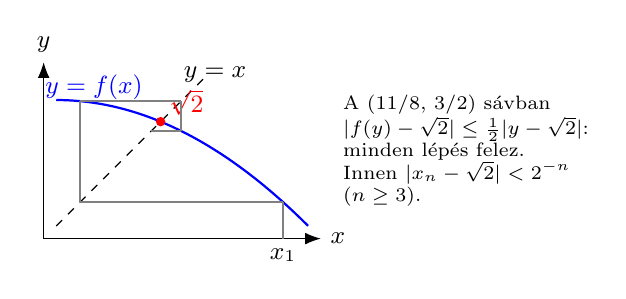
\begin{tikzpicture}[font=\small,scale=3.2]
  \draw[nyil] (0.95,0.95) -- (2.05,0.95) node[right] {$x$};
  \draw[nyil] (0.95,0.95) -- (0.95,1.65) node[above] {$y$};
  \draw[domain=1:2,samples=80,thick,blue] plot (\x,{-\x*\x/2+\x+1});
  \node[blue] at (1.15,1.55) {$y=f(x)$};
  \draw[domain=1:1.6,samples=2,dashed] plot (\x,\x);
  \node at (1.63,1.6) {$y=x$};
  \node[pont,red] at (1.41421,1.41421) {}; \node[red,above right] at (1.41,1.40) {$\sqrt2$};
  % cobweb from x0 = 1.9
  \draw[thick,gray] (1.9,0.95) -- (1.9,1.095);
  \draw[thick,gray] (1.9,1.095) -- (1.095,1.095);
  \draw[thick,gray] (1.095,1.095) -- (1.095,1.495);
  \draw[thick,gray] (1.095,1.495) -- (1.495,1.495);
  \draw[thick,gray] (1.495,1.495) -- (1.495,1.377);
  \draw[thick,gray] (1.495,1.377) -- (1.377,1.377);
  \node[below] at (1.9,0.95) {$x_1$};
  \node[anchor=west,align=left,font=\scriptsize] at (2.1,1.3)
    {A $(11/8,\,3/2)$ sávban\\ $|f(y)-\sqrt2| \le \tfrac12|y-\sqrt2|$:\\
     minden lépés felez.\\ Innen $|x_n-\sqrt2|<2^{-n}$\\ ($n\ge3$).};
\end{tikzpicture}
\end{center}

\noindent Lean: \lean{Kalkulus1.Rajzok.pokhalo\_zsugorodas} (általános zsugorítás) és
\lean{Kalkulus1.Rajzok.gyak\_1\_18} (maga a feladat).

\section{Határérték és folytonosság}

\subsection{Az $\eps$--$\delta$ doboz (3.1)}

\begin{center}
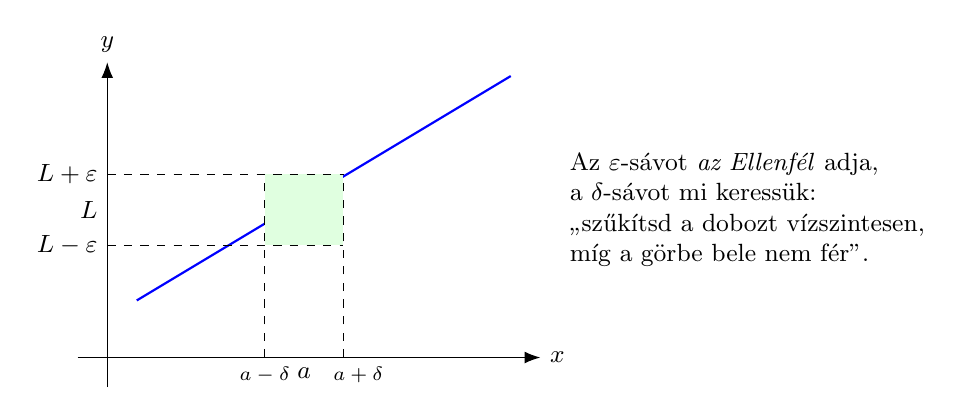
\begin{tikzpicture}[font=\small,scale=1.25]
  \draw[nyil] (-0.3,0) -- (4.4,0) node[right] {$x$};
  \draw[nyil] (0,-0.3) -- (0,3.0) node[above] {$y$};
  \draw[domain=0.3:4.1,samples=80,thick,blue] plot (\x,{0.6*\x+0.4});
  \fill[green!12] (1.6,1.14) rectangle (2.4,1.86);
  \draw[dashed] (0,1.14) -- (2.4,1.14); \draw[dashed] (0,1.86) -- (2.4,1.86);
  \draw[dashed] (1.6,0) -- (1.6,1.86); \draw[dashed] (2.4,0) -- (2.4,1.86);
  \node[left] at (0,1.5) {$L$}; \node[left] at (0,1.86) {$L+\eps$};
  \node[left] at (0,1.14) {$L-\eps$};
  \node[below] at (2,0) {$a$};
  \node[below] at (1.6,0) {\scriptsize $a-\delta$}; \node[below] at (2.55,0) {\scriptsize $a+\delta$};
  \node[anchor=west,align=left] at (4.6,1.5)
    {Az $\eps$-sávot \emph{az Ellenfél} adja,\\ a $\delta$-sávot mi keressük:\\
     „szűkítsd a dobozt vízszintesen,\\ míg a görbe bele nem fér”.};
\end{tikzpicture}
\end{center}

\subsection{A végtelenben: melyik tag dominál (3.2, 3.3)}\label{fig:dominans}

Racionális törtnél osszunk a nevező legmagasabb fokú tagjával --- a rajzon ez azt
jelenti, hogy „messziről nézve” minden tag eltűnik a domináns mellett. Három eset van,
és mindhármat egy-egy vázlat rögzíti.

\begin{center}
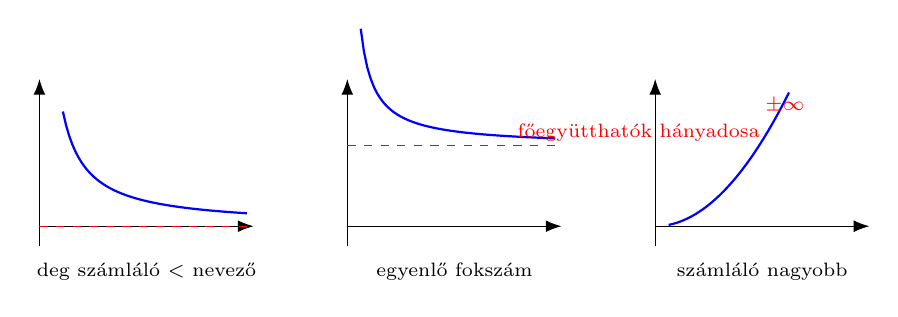
\begin{tikzpicture}[font=\small,scale=0.85]
  \foreach \i/\lab/\ex in {0/{$\deg$ számláló $<$ nevező}/{0}, 4.6/{egyenlő fokszám}/{1}, 9.2/{számláló nagyobb}/{2}} {
    \begin{scope}[xshift=\i cm]
      \draw[nyil] (0,0) -- (3.2,0); \draw[nyil] (0,-0.3) -- (0,2.2);
      \node[below,font=\scriptsize,align=center] at (1.6,-0.4) {\lab};
    \end{scope}
  }
  \draw[domain=0.35:3.1,samples=60,thick,blue] plot (\x,{0.6/\x});
  \draw[dashed,red] (0,0) -- (3.2,0);
  \begin{scope}[xshift=4.6cm]
    \draw[domain=0.2:3.1,samples=60,thick,blue] plot (\x,{1.2+0.35/\x});
    \draw[dashed,red] (0,1.2) -- (3.2,1.2); \node[right,font=\scriptsize,red] at (2.4,1.4) {főegyütthatók hányadosa};
  \end{scope}
  \begin{scope}[xshift=9.2cm]
    \draw[domain=0.2:2.0,samples=60,thick,blue] plot (\x,{0.5*\x*\x});
    \node[right,font=\scriptsize,red] at (1.5,1.8) {$\pm\infty$};
  \end{scope}
\end{tikzpicture}
\end{center}

\begin{fogas}[gyöktelenítés, 3.3 f--h]
A $\sqrt{x^2+x}-\sqrt{x^2-x}$ típusú kifejezés rajza: két, egymáshoz nagyon közeli görbe
\emph{függőleges} távolsága. Ilyenkor a különbséget szorozzuk-osszuk az összeggel:
a rajzon ez azt jelenti, hogy a keskeny rést a két görbe \emph{összegével} mérjük,
ami már nem tűnik el. Negatív $x$ esetén ne feledjük: $\sqrt{x^2}=|x|=-x$.
\end{fogas}

\subsection{$0/0$: lyuk a grafikonon (3.4, 3.12)}

A $\frac{x^2-4}{x-2}$ függvény grafikonja az $y=x+2$ egyenes egy \emph{kilyukasztott}
ponttal. A határérték a lyuk „magassága” --- a megszüntethető szakadás pontosan ez.

\begin{center}
\begin{tikzpicture}[font=\small,scale=0.8]
  \draw[nyil] (-0.4,0) -- (4.4,0) node[right] {$x$};
  \draw[nyil] (0,-0.4) -- (0,5.2) node[above] {$y$};
  \draw[domain=-0.3:3.2,samples=2,thick,blue] plot (\x,{\x+2});
  \node[ures,blue] at (2,4) {};
  \draw[dashed] (2,0) -- (2,4); \draw[dashed] (0,4) -- (2,4);
  \node[below] at (2,0) {$2$}; \node[left] at (0,4) {$4$};
  \node[anchor=west,align=left] at (4.6,2.6)
    {$h(2):=4$ betöltése után\\ a függvény folytonos (3.12 a).};
\end{tikzpicture}
\end{center}

\subsection{A szakadások három arca (3.11)}

\begin{center}
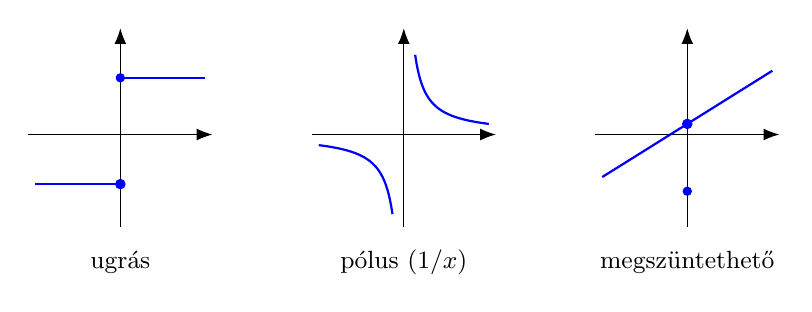
\begin{tikzpicture}[font=\small,scale=0.9]
  \begin{scope}
    \draw[nyil] (-1.3,0) -- (1.3,0); \draw[nyil] (0,-1.3) -- (0,1.5);
    \draw[thick,blue] (-1.2,-0.7) -- (-0.05,-0.7);
    \draw[thick,blue] (0.05,0.8) -- (1.2,0.8);
    \node[ures,blue] at (0,-0.7) {}; \node[pont,blue] at (0,0.8) {};
    \node at (0,-1.8) {ugrás};
  \end{scope}
  \begin{scope}[xshift=4cm]
    \draw[nyil] (-1.3,0) -- (1.3,0); \draw[nyil] (0,-1.3) -- (0,1.5);
    \draw[domain=0.16:1.2,samples=60,thick,blue] plot (\x,{0.18/\x});
    \draw[domain=-1.2:-0.16,samples=60,thick,blue] plot (\x,{0.18/\x});
    \node at (0,-1.8) {pólus ($1/x$)};
  \end{scope}
  \begin{scope}[xshift=8cm]
    \draw[nyil] (-1.3,0) -- (1.3,0); \draw[nyil] (0,-1.3) -- (0,1.5);
    \draw[thick,blue] (-1.2,-0.6) -- (1.2,0.9);
    \node[ures,blue] at (0,0.15) {}; \node[pont,blue] at (0,-0.8) {};
    \node at (0,-1.8) {megszüntethető};
  \end{scope}
\end{tikzpicture}
\end{center}

\noindent A 3.11 feladat rajza után a b)--d) kérdésekre a válasz \emph{leolvasható};
a papíron csak a leolvasottat kell egyenlőtlenségekké fordítani.

\subsection{Illesztés paraméterrel (3.13, 4.7)}

Egy paraméter, egy feltétel: a folytonossághoz a két görbedarabnak \emph{találkoznia}
kell az illesztési pontban. Ha a differenciálhatóságot is kérjük (4.7), az egy második
feltétel: a meredekségek is egyeznek. Rajz: két ceruzavonal, amit „össze kell hegeszteni”.

\begin{center}
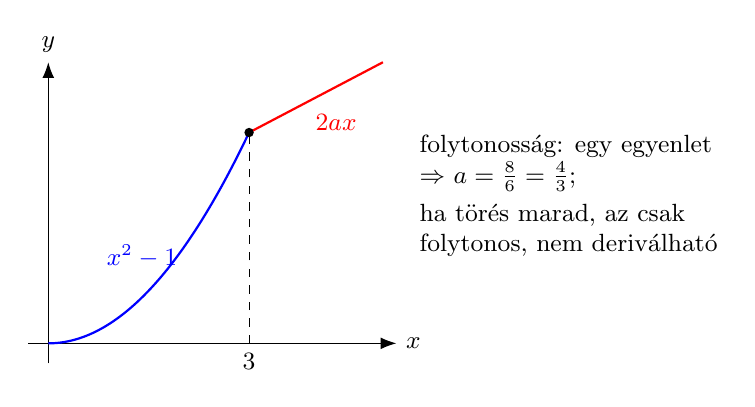
\begin{tikzpicture}[font=\small,scale=0.85]
  \draw[nyil] (-0.3,0) -- (5.2,0) node[right] {$x$};
  \draw[nyil] (0,-0.3) -- (0,4.2) node[above] {$y$};
  \draw[domain=0:3,samples=60,thick,blue] plot (\x,{0.35*\x*\x});
  \draw[thick,red] (3,3.15) -- (5,4.2);
  \node[pont] at (3,3.15) {};
  \draw[dashed] (3,0) -- (3,3.15); \node[below] at (3,0) {$3$};
  \node[blue] at (1.4,1.3) {$x^2-1$};
  \node[red] at (4.3,3.3) {$2ax$};
  \node[anchor=west,align=left] at (5.4,2.2)
    {folytonosság: egy egyenlet\\ $\Rightarrow$ $a=\frac{8}{6}=\frac43$;\\[1mm]
     ha törés marad, az csak\\ folytonos, nem deriválható};
\end{tikzpicture}
\end{center}

\subsection{Monoton és korlátos (3.14) --- a plafon-rajz}

Ha $f$ monoton nő és felülről korlátos, akkor az értékek egy plafonhoz \emph{felgyűlnek}:
a bal oldali határérték a képhalmaz szuprémuma. A bizonyítás rajza: a $\sup$-hoz húzunk
egy $\eps$-sávot, és a szuprémum definíciója szerint van olyan pont, ahol már belépünk a sávba;
a monotonitás miatt onnantól benne is maradunk.

\begin{center}
\begin{tikzpicture}[font=\small,scale=1.0]
  \draw[nyil] (-0.2,0) -- (5.2,0) node[right] {$x$};
  \draw[nyil] (0,-0.2) -- (0,3.0) node[above] {$y$};
  \draw[domain=0.1:4.6,samples=80,thick,blue] plot (\x,{2.2-1.6/(\x+0.7)});
  \draw[dashed,red] (0,2.2) -- (5.0,2.2); \node[right,red] at (4.6,2.4) {$M=\sup$};
  \draw[dashed] (0,1.95) -- (5.0,1.95); \node[left,font=\scriptsize] at (0,1.95) {$M-\eps$};
  \draw[dotted] (4.7,0) -- (4.7,2.3); \node[below] at (4.7,0) {$b$};
  \node[pont] at (3.05,1.95) {};
  \node[anchor=west,align=left,font=\scriptsize] at (5.4,1.3)
    {van $x_0$, ahol $f(x_0)>M-\eps$;\\ $x>x_0$ esetén $f(x)\in(M-\eps,M]$.};
\end{tikzpicture}
\end{center}

\subsection{Sűrűség: két folytonos függvény a racionálisokon (3.15)}

Rajzoljuk a racionális pontokat „sűrű fésűként” a tengelyre: ha a két grafikon minden
fogon találkozik, akkor a folytonosság miatt sehol sem tud szétválni --- egy irracionális
$x$-hez ugyanis racionális sorozat tart, és a függvényértékek követik.

\begin{center}
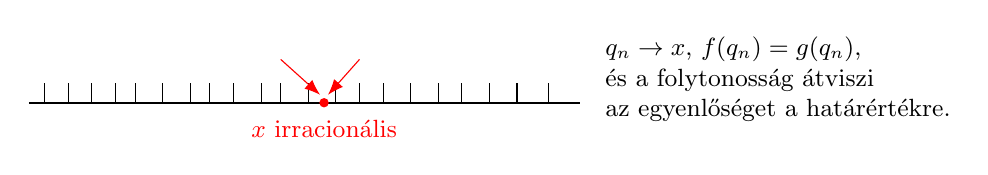
\begin{tikzpicture}[font=\small,scale=1.0]
  \draw[seg] (0,0) -- (7,0);
  \foreach \x in {0.2,0.5,0.8,1.1,1.35,1.7,2.05,2.3,2.6,2.95,3.2,3.55,3.9,4.2,4.5,4.85,5.2,5.5,5.85,6.2,6.6}
    \draw (\x,0) -- (\x,0.25);
  \node[pont,red] at (3.75,0) {}; \node[below,red] at (3.75,-0.1) {$x$ irracionális};
  \draw[nyil,red] (3.2,0.55) -- (3.7,0.1);
  \draw[nyil,red] (4.2,0.55) -- (3.8,0.1);
  \node[anchor=west,align=left] at (7.2,0.3)
    {$q_n\to x$, $f(q_n)=g(q_n)$,\\ és a folytonosság átviszi\\ az egyenlőséget a határértékre.};
\end{tikzpicture}
\end{center}

\subsection{Az egységkör-szendvics (3.7) és az $e$ (3.10, 3.16)}

\begin{center}
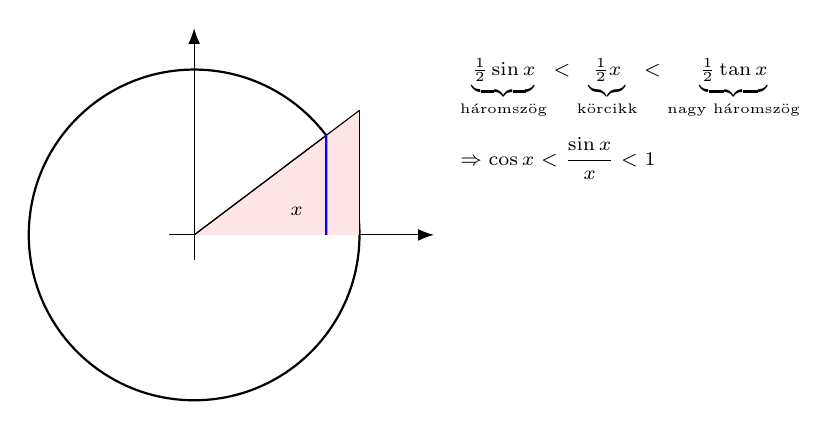
\begin{tikzpicture}[font=\small,scale=2.1]
  \draw[nyil] (-0.15,0) -- (1.45,0); \draw[nyil] (0,-0.15) -- (0,1.25);
  \draw[thick] (0,0) circle (1);
  \coordinate (O) at (0,0);
  \coordinate (A) at (1,0);
  \coordinate (P) at (37:1);
  \coordinate (T) at (1,{tan(37)});
  \fill[blue!14] (O) -- (A) -- (P) -- cycle;
  \fill[red!10] (A) -- (T) -- (O) -- cycle;
  \draw (O) -- (P); \draw (O) -- (T); \draw (A) -- (T);
  \draw[thick,blue] (P) -- ({cos(37)},0);
  \node[anchor=west,align=left,font=\scriptsize] at (1.55,0.7)
    {$\underbrace{\tfrac12\sin x}_{\text{háromszög}} <
      \underbrace{\tfrac12 x}_{\text{körcikk}} <
      \underbrace{\tfrac12\tan x}_{\text{nagy háromszög}}$\\[2mm]
     $\Rightarrow \cos x < \dfrac{\sin x}{x} < 1$};
  \node[font=\scriptsize] at (0.62,0.14) {$x$};
\end{tikzpicture}
\end{center}

\noindent Lean: \lean{Kalkulus1.Rajzok.egysegkor\_szendvics}, \lean{rendorelv\_sav}.
Az $\left(1+\frac1n\right)^n$ sorozathoz (3.10, 3.16) a rajz a hiperbola alatti terület:
$\ln(1+t)$ a $1/x$ görbe alatti terület $1$-től $1+t$-ig, és a beírt/körülírt téglalap adja a
$\frac{t}{1+t} < \ln(1+t) < t$ becslést --- ebből a monotonitás és a korlátosság is kijön.

\begin{center}
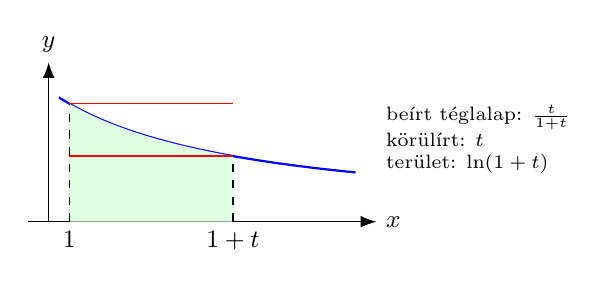
\begin{tikzpicture}[font=\small,xscale=2.6,yscale=1.5]
  \draw[nyil] (0.8,0) -- (2.5,0) node[right] {$x$};
  \draw[nyil] (0.9,0) -- (0.9,1.35) node[above] {$y$};
  \draw[domain=0.95:2.4,samples=80,thick,blue] plot (\x,{1/\x});
  \fill[green!12,domain=1:1.8,variable=\x] (1,0) -- plot (\x,{1/\x}) -- (1.8,0) -- cycle;
  \draw[dashed] (1,0) -- (1,1); \draw[dashed] (1.8,0) -- (1.8,0.556);
  \draw[red] (1,0.556) -- (1.8,0.556);
  \draw[red] (1,1) -- (1.8,1);
  \node[below] at (1,0) {$1$}; \node[below] at (1.8,0) {$1+t$};
  \node[anchor=west,align=left,font=\scriptsize] at (2.5,0.7)
    {beírt téglalap: $\frac{t}{1+t}$\\ körülírt: $t$\\
     terület: $\ln(1+t)$};
\end{tikzpicture}
\end{center}

\section{Derivált és alkalmazásai}

\subsection{Szelő $\to$ érintő (4.1)}

\begin{center}
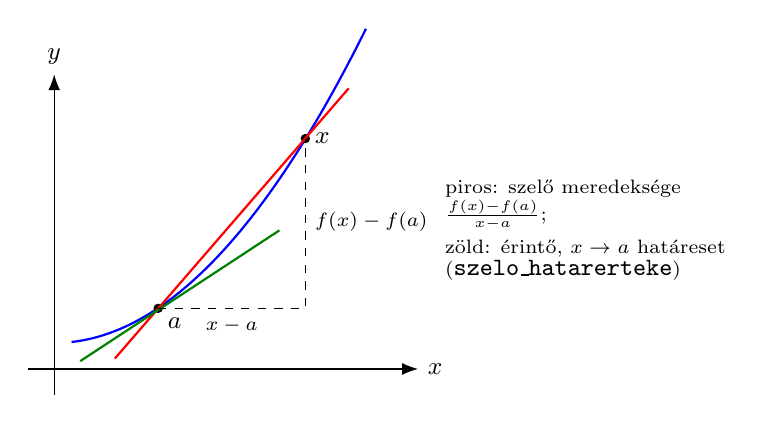
\begin{tikzpicture}[font=\small,scale=1.1]
  \draw[nyil] (-0.3,0) -- (4.2,0) node[right] {$x$};
  \draw[nyil] (0,-0.3) -- (0,3.4) node[above] {$y$};
  \draw[domain=0.2:3.6,samples=80,thick,blue] plot (\x,{0.28*\x*\x+0.3});
  \node[pont] at (1.2,0.70) {}; \node[below right] at (1.2,0.70) {$a$};
  \node[pont] at (2.9,2.66) {}; \node[right] at (2.9,2.66) {$x$};
  \draw[red,thick] (0.7,0.12) -- (3.4,3.24);
  \draw[green!50!black,thick] (0.3,0.09) -- (2.6,1.6);
  \draw[dashed] (1.2,0.70) -- (2.9,0.70) -- (2.9,2.66);
  \node[below,font=\scriptsize] at (2.05,0.70) {$x-a$};
  \node[right,font=\scriptsize] at (2.9,1.7) {$f(x)-f(a)$};
  \node[anchor=west,align=left,font=\scriptsize] at (4.4,1.6)
    {piros: szelő meredeksége\\ $\frac{f(x)-f(a)}{x-a}$;\\[1mm]
     zöld: érintő, $x\to a$ határeset\\ (\lean{szelo\_hatarerteke})};
\end{tikzpicture}
\end{center}

\subsection{A nem differenciálhatóság négy tipikus képe (4.4, 4.5)}

\begin{center}
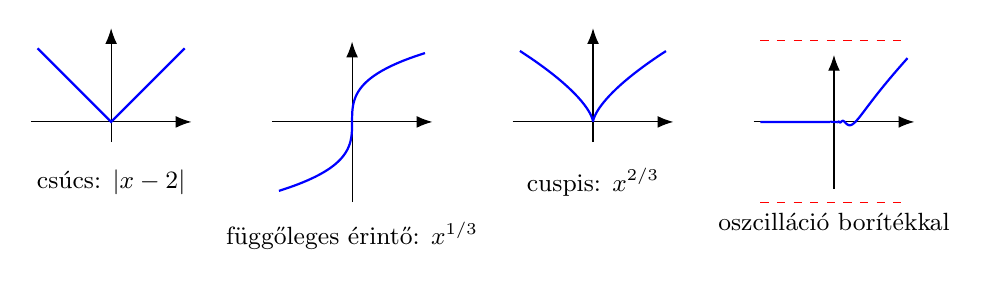
\begin{tikzpicture}[font=\small,scale=0.85]
  \begin{scope}
    \draw[nyil] (-1.2,0) -- (1.2,0); \draw[nyil] (0,-0.3) -- (0,1.4);
    \draw[thick,blue] (-1.1,1.1) -- (0,0) -- (1.1,1.1);
    \node at (0,-0.9) {csúcs: $|x-2|$};
  \end{scope}
  \begin{scope}[xshift=3.6cm]
    \draw[nyil] (-1.2,0) -- (1.2,0); \draw[nyil] (0,-1.2) -- (0,1.2);
    \draw[domain=-1.03:1.03,samples=80,variable=\t,thick,blue] plot ({\t*\t*\t},{\t});
    \node at (0,-1.7) {függőleges érintő: $x^{1/3}$};
  \end{scope}
  \begin{scope}[xshift=7.2cm]
    \draw[nyil] (-1.2,0) -- (1.2,0); \draw[nyil] (0,-0.3) -- (0,1.4);
    \draw[domain=-1.03:1.03,samples=80,variable=\t,thick,blue] plot ({\t*\t*\t},{\t*\t});
    \node at (0,-0.9) {cuspis: $x^{2/3}$};
  \end{scope}
  \begin{scope}[xshift=10.8cm]
    \draw[nyil] (-1.2,0) -- (1.2,0); \draw[nyil] (0,-1.0) -- (0,1.0);
    \draw[domain=0.055:1.1,samples=400,thick,blue] plot (\x,{\x*\x*sin(1/\x r)});
    \draw[domain=-1.1:-0.055,samples=400,thick,blue] plot (\x,{\x*\x*sin(1/\x r)});
    \draw[thick,blue] (-0.055,0.0016) -- (0,0) -- (0.055,-0.0016);
    \draw[dashed,red,domain=-1.1:1.1,samples=2] plot (\x,{\x*\x});
    \draw[dashed,red,domain=-1.1:1.1,samples=2] plot (\x,{-\x*\x});
    \node at (0,-1.5) {oszcilláció boríték\-kal};
  \end{scope}
\end{tikzpicture}
\end{center}

\noindent A negyedik kép azt is megmutatja, \emph{miért} deriválható mégis a
$x^2\sin(1/x)$ függvény a $0$-ban: a $\pm x^2$ boríték a különbségi hányadost
$\pm|x|$ közé szorítja --- rendőrelv (4.5 e).

\subsection{Láncszabály: két fogaskerék (4.2)}

A láncszabály rajza két összekapcsolt fogaskerék (vagy két egymás utáni sebességváltó):
ha a belső $u$ háromszor olyan gyorsan változik, mint $x$, és a külső $y$ ötször olyan
gyorsan, mint $u$, akkor $y$ tizenötször olyan gyorsan, mint $x$.

\begin{center}
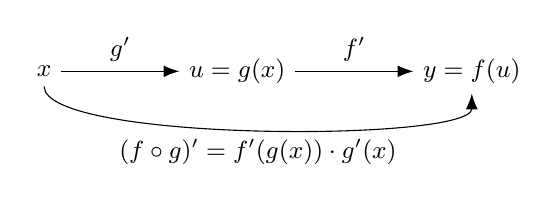
\begin{tikzpicture}[font=\small,node distance=15mm]
  \node (x) {$x$}; \node (u) [right=of x] {$u=g(x)$}; \node (y) [right=of u] {$y=f(u)$};
  \draw[nyil] (x) -- node[above] {$g'$} (u);
  \draw[nyil] (u) -- node[above] {$f'$} (y);
  \draw[nyil] (x) .. controls +(0,-9mm) and +(0,-9mm) .. node[below] {$(f\circ g)' = f'(g(x))\cdot g'(x)$} (y);
\end{tikzpicture}
\end{center}

\subsection{Logaritmikus deriválás: relatív változás (4.3)}

$\bigl(\ln f\bigr)' = f'/f$: a logaritmus a \emph{relatív} (százalékos) változást méri.
Ezért lesz szorzatból összeg, hatványból szorzat --- a rajzon a log-skálás papír képe:
a szorzótényezők egymás fölé rakódnak.

\begin{center}
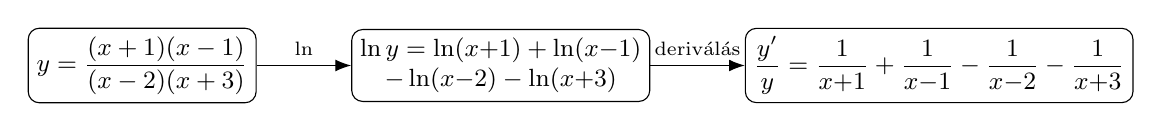
\begin{tikzpicture}[font=\small]
  \node[dob] (a) {$y=\dfrac{(x+1)(x-1)}{(x-2)(x+3)}$};
  \node[dob,right=12mm of a] (b) {$\ln y = \ln(x{+}1)+\ln(x{-}1)$\\ $-\ln(x{-}2)-\ln(x{+}3)$};
  \node[dob,right=12mm of b] (c) {$\dfrac{y'}{y}=\dfrac{1}{x{+}1}+\dfrac{1}{x{-}1}-\dfrac{1}{x{-}2}-\dfrac{1}{x{+}3}$};
  \draw[nyil] (a) -- node[above,font=\scriptsize] {$\ln$} (b);
  \draw[nyil] (b) -- node[above,font=\scriptsize] {deriválás} (c);
\end{tikzpicture}
\end{center}

\subsection{Menetvizsgálat: négy alapikon (4.8)}

Az $f'$ és $f''$ előjelének négy kombinációja négy ceruzavonás. A teljes menetvizsgálat
nem más, mint ezeknek az ikonoknak az összefűzése az előjelvonal szerint.

\begin{center}
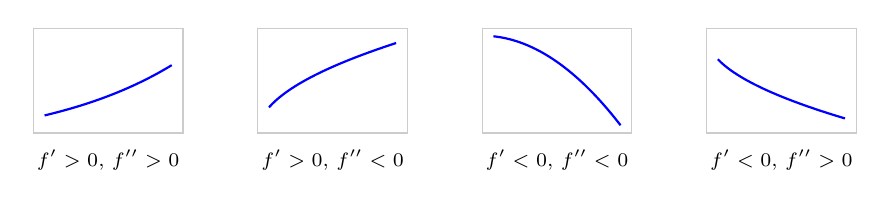
\begin{tikzpicture}[font=\small,scale=0.95]
  \foreach \i/\lab/\opt in {0/{$f'>0$, $f''>0$}/a, 3/{$f'>0$, $f''<0$}/b,
                            6/{$f'<0$, $f''<0$}/c, 9/{$f'<0$, $f''>0$}/d} {
    \begin{scope}[xshift=\i cm]
      \draw[gray!40] (0,0) rectangle (2,1.4);
      \node[below,font=\scriptsize,align=center] at (1,-0.1) {\lab};
    \end{scope}
  }
  \draw[thick,blue,domain=0.15:1.85,samples=40] plot (\x,{0.4*exp(0.55*\x)-0.2});
  \begin{scope}[xshift=3cm]
    \draw[thick,blue,domain=0.15:1.85,samples=40] plot (\x,{1.25*sqrt(\x/2)});
  \end{scope}
  \begin{scope}[xshift=6cm]
    \draw[thick,blue,domain=0.15:1.85,samples=40] plot (\x,{1.3-0.35*\x*\x});
  \end{scope}
  \begin{scope}[xshift=9cm]
    \draw[thick,blue,domain=0.15:1.85,samples=40] plot (\x,{1.3-1.15*sqrt(\x/2)});
  \end{scope}
\end{tikzpicture}
\end{center}

\subsection{Abszolút szélsőérték: a gyanúsítottak listája (4.9)}

Zárt intervallumon három helyen lehet abszolút szélsőérték: ahol $f'=0$, ahol $f'$ nem
létezik, és a végpontokban. A rajz: karikázzuk be mind a hármat, majd hasonlítsunk értéket.

\begin{center}
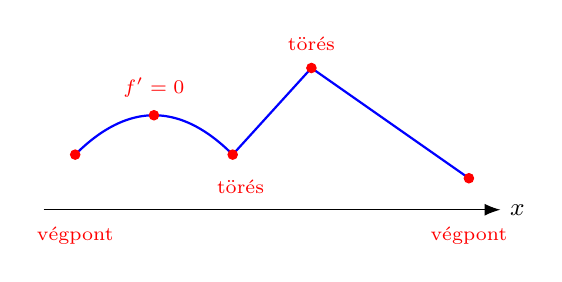
\begin{tikzpicture}[font=\small,scale=1.0]
  \draw[nyil] (-0.4,0) -- (5.4,0) node[right] {$x$};
  \draw[thick,blue,domain=0:2,samples=60] plot (\x,{1.2-0.5*(\x-1)*(\x-1)});
  \draw[thick,blue] (2,0.7) -- (3,1.8);
  \draw[thick,blue,domain=3:5,samples=60] plot (\x,{1.8-0.7*(\x-3)});
  \node[ures,red] at (0,0.7) {}; \node[below,font=\scriptsize,red] at (0,-0.1) {végpont};
  \node[ures,red] at (1,1.2) {}; \node[above,font=\scriptsize,red] at (1,1.3) {$f'=0$};
  \node[ures,red] at (2,0.7) {}; \node[below,font=\scriptsize,red] at (2.1,0.5) {törés};
  \node[ures,red] at (3,1.8) {}; \node[above,font=\scriptsize,red] at (3,1.9) {törés};
  \node[ures,red] at (5,0.4) {}; \node[below,font=\scriptsize,red] at (5,-0.1) {végpont};
\end{tikzpicture}
\end{center}

\subsection{L'Hospital: két linearizálás hányadosa (4.10)}

A $0/0$ alak rajza: mindkét görbe átmegy az origón, és közel hozzá az érintőikkel
helyettesíthetők. A hányados határértéke ezért a két meredekség hányadosa --- ez a
L'Hospital-szabály képe (és egyben a helyes használat feltétele: mindkét függvény
menjen nullába).

\begin{center}
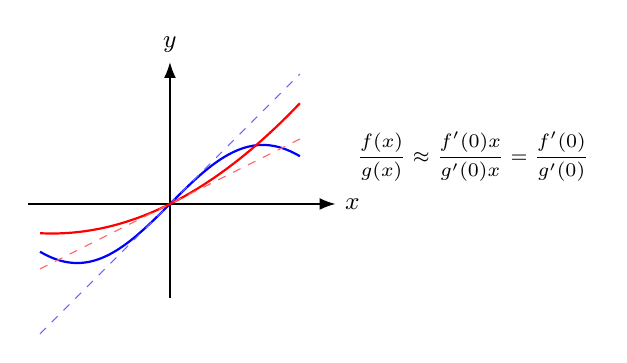
\begin{tikzpicture}[font=\small,scale=1.5]
  \draw[nyil] (-1.2,0) -- (1.4,0) node[right] {$x$};
  \draw[nyil] (0,-0.8) -- (0,1.2) node[above] {$y$};
  \draw[domain=-1.1:1.1,samples=80,thick,blue] plot (\x,{sin(2*\x r)/2});
  \draw[dashed,blue!60] (-1.1,-1.1) -- (1.1,1.1);
  \draw[domain=-1.1:1.1,samples=80,thick,red] plot (\x,{0.5*\x+0.25*\x*\x});
  \draw[dashed,red!60] (-1.1,-0.55) -- (1.1,0.55);
  \node[anchor=west,align=left,font=\scriptsize] at (1.5,0.4)
    {$\dfrac{f(x)}{g(x)} \approx \dfrac{f'(0)x}{g'(0)x} = \dfrac{f'(0)}{g'(0)}$};
\end{tikzpicture}
\end{center}

\subsection{Optimalizálás geometriája (4.11, 4.12, 4.14, 4.15)}

A szöveges szélsőérték-feladatoknál a rajz \emph{kötelező}, mert belőle olvassuk ki a
kényszert (kerület, terület, a parabola alatti fekvés), és belőle látszik, melyik
változó fejezhető ki a másikkal. Utána egyváltozós feladat marad.

\begin{center}
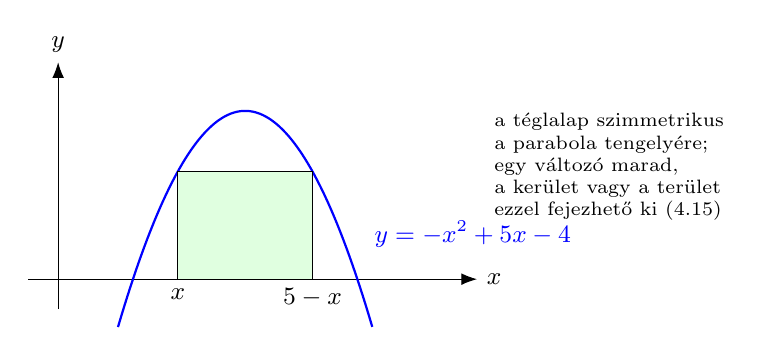
\begin{tikzpicture}[font=\small,scale=0.95]
  \draw[nyil] (-0.4,0) -- (5.6,0) node[right] {$x$};
  \draw[nyil] (0,-0.4) -- (0,2.9) node[above] {$y$};
  \draw[domain=0.8:4.2,samples=80,thick,blue] plot (\x,{-(\x*\x)+5*\x-4});
  \node[blue,anchor=west] at (4.1,0.6) {$y=-x^2+5x-4$};
  \draw[fill=green!12] (1.6,0) rectangle (3.4,{-(1.6*1.6)+5*1.6-4});
  \node[below] at (1.6,0) {$x$}; \node[below] at (3.4,0) {$5-x$};
  \node[anchor=west,align=left,font=\scriptsize] at (5.7,1.5)
    {a téglalap szimmetrikus\\ a parabola tengelyére;\\
     egy változó marad,\\ a kerület vagy a terület\\ ezzel fejezhető ki (4.15)};
\end{tikzpicture}
\end{center}

\subsection{Középponti konvexitás (4.13): felezéses finomítás}

A feltétel a felezőpontra szól; a rajz mutatja, hogyan terjed ki minden diadikus arányra
($1/2$, $1/4$, $3/8$, \dots), majd a folytonosság „kitölti a lyukakat”.

\begin{center}
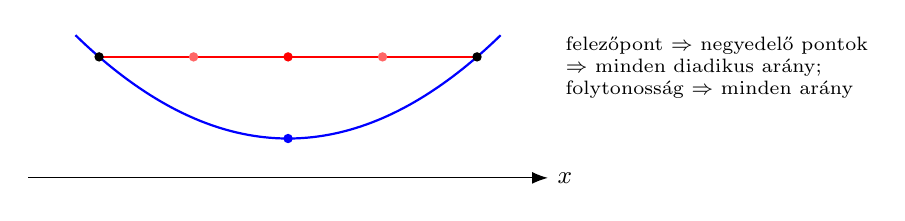
\begin{tikzpicture}[font=\small,scale=1.0]
  \draw[nyil] (-0.3,0) -- (6.3,0) node[right] {$x$};
  \draw[domain=0.3:5.7,samples=80,thick,blue] plot (\x,{0.18*(\x-3)*(\x-3)+0.5});
  \coordinate (A) at (0.6,{0.18*(0.6-3)*(0.6-3)+0.5});
  \coordinate (B) at (5.4,{0.18*(5.4-3)*(5.4-3)+0.5});
  \draw[red,thick] (A) -- (B);
  \node[pont] at (A) {}; \node[pont] at (B) {};
  \foreach \x in {3} {
    \node[pont,red] at (\x,{0.5*(0.18*(0.6-3)*(0.6-3)+0.5)+0.5*(0.18*(5.4-3)*(5.4-3)+0.5)}) {};
    \node[pont,blue] at (\x,{0.18*(\x-3)*(\x-3)+0.5}) {};
  }
  \foreach \x in {1.8,4.2} {
    \node[pont,red!60] at (\x,{0.18*(0.6-3)*(0.6-3)+0.5 + (\x-0.6)/4.8*((0.18*(5.4-3)*(5.4-3)+0.5)-(0.18*(0.6-3)*(0.6-3)+0.5))}) {};
  }
  \node[anchor=west,align=left,font=\scriptsize] at (6.4,1.4)
    {felezőpont $\Rightarrow$ negyedelő pontok\\ $\Rightarrow$ minden diadikus arány;\\
     folytonosság $\Rightarrow$ minden arány};
\end{tikzpicture}
\end{center}

\section{Kategóriaelméleti diagramok: a nyilak nyelve}

A kategóriaelméleti rajz ugyanaz a ceruzamozdulat, mint a halmazos nyíldiagram, csak
következetesebb: \emph{objektumok} pontok, \emph{morfizmusok} nyilak, és a lényeg mindig
az, hogy két út ugyanoda vezet-e (\emph{kommutál-e} a diagram).

\begin{center}
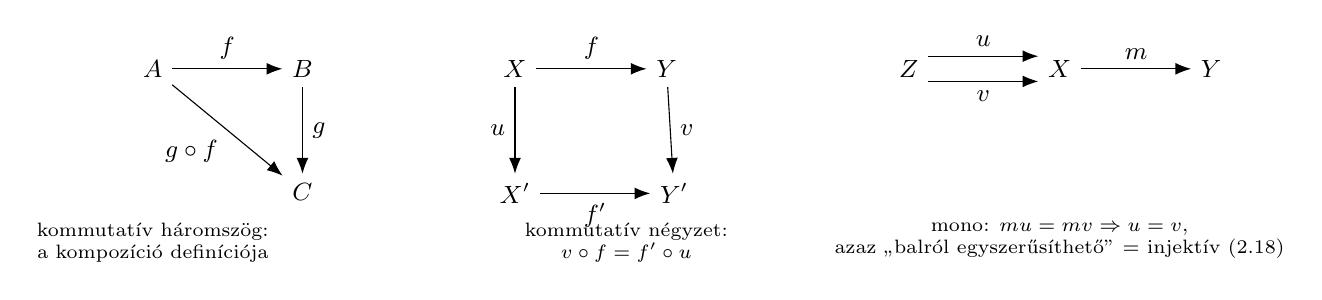
\begin{tikzpicture}[font=\small,node distance=14mm]
  \begin{scope}
    \node (A) {$A$}; \node (B) [right=of A] {$B$};
    \node (C) [below=11mm of B] {$C$};
    \draw[nyil] (A) -- node[above] {$f$} (B);
    \draw[nyil] (B) -- node[right] {$g$} (C);
    \draw[nyil] (A) -- node[below left] {$g\circ f$} (C);
    \node[below=16mm of A,align=center,font=\scriptsize] {kommutatív háromszög:\\ a kompozíció definíciója};
  \end{scope}
  \begin{scope}[xshift=4.6cm]
    \node (A) {$X$}; \node (B) [right=of A] {$Y$};
    \node (C) [below=11mm of A] {$X'$}; \node (D) [right=of C] {$Y'$};
    \draw[nyil] (A) -- node[above] {$f$} (B);
    \draw[nyil] (A) -- node[left] {$u$} (C);
    \draw[nyil] (B) -- node[right] {$v$} (D);
    \draw[nyil] (C) -- node[below] {$f'$} (D);
    \node[below=16mm of A,anchor=north west,align=center,font=\scriptsize]
      {kommutatív négyzet:\\ $v\circ f = f'\circ u$};
  \end{scope}
  \begin{scope}[xshift=9.6cm]
    \node (Z) {$Z$}; \node (A) [right=of Z] {$X$}; \node (B) [right=of A] {$Y$};
    \draw[nyil,transform canvas={yshift=1.6mm}] (Z) -- node[above] {$u$} (A);
    \draw[nyil,transform canvas={yshift=-1.6mm}] (Z) -- node[below] {$v$} (A);
    \draw[nyil] (A) -- node[above] {$m$} (B);
    \node[below=16mm of A,align=center,font=\scriptsize]
      {mono: $m u = m v \Rightarrow u=v$,\\ azaz „balról egyszerűsíthető” $=$ injektív (2.18)};
  \end{scope}
\end{tikzpicture}
\end{center}

\subsection{A szuprémum univerzális tulajdonsága (1.4, 1.5)}

Rendezett halmazban a nyíl a $\le$ reláció. Ekkor a $\sup S$ nem más, mint az
\emph{univerzális} felső korlát: minden felső korlát felette van. Ebből az
egyértelműség egy soros: két univerzális objektum között oda-vissza nyíl fut.

\begin{center}
\begin{tikzpicture}[font=\small,node distance=13mm]
  \node (s) {$S$};
  \node (sup) [above right=8mm and 14mm of s] {$\sup S$};
  \node (m) [above right=8mm and 14mm of sup] {$M$ (bármely felső korlát)};
  \draw[nyil] (s) -- node[below right,font=\scriptsize] {$\le$} (sup);
  \draw[nyil] (sup) -- node[below right,font=\scriptsize] {$\le$} (m);
  \draw[nyil,dashed] (s) .. controls +(0,12mm) and +(-14mm,6mm) .. node[above,font=\scriptsize] {$\le$} (m);
\end{tikzpicture}
\end{center}

\subsection{Galois-kapcsolat: két oszlop, oda-vissza nyíl}

Az egészrész és a beágyazás kapcsolata ($z \le x \iff z \le \lfloor x\rfloor$, $z\in\Z$),
a $\sup$ és a konstans-halmaz kapcsolata, a „legkisebb felső korlát” --- mind ugyanaz a
kép: két rendezett halmaz, oda-vissza egy-egy monoton nyíl, és a megfelelés
\emph{szintenként} olvasható le.

\begin{center}
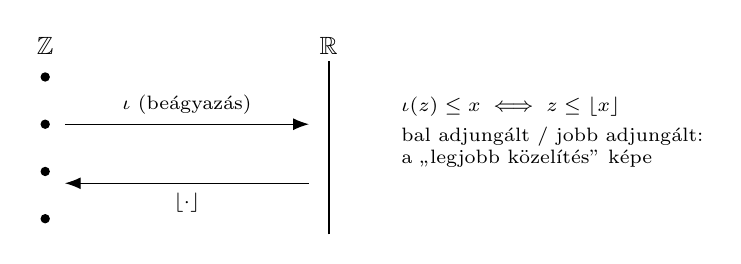
\begin{tikzpicture}[font=\small]
  \node at (0,2.2) {$\Z$}; \node at (3.6,2.2) {$\R$};
  \foreach \y in {0,0.6,1.2,1.8} {\node[pont] at (0,\y) {}; }
  \draw[seg] (3.6,-0.2) -- (3.6,2.0);
  \draw[nyil] (0.25,1.2) -- node[above,font=\scriptsize] {$\iota$ (beágyazás)} (3.35,1.2);
  \draw[nyil] (3.35,0.45) -- node[below,font=\scriptsize] {$\lfloor\cdot\rfloor$} (0.25,0.45);
  \node[anchor=west,align=left,font=\scriptsize] at (4.4,1.1)
    {$\iota(z) \le x \iff z \le \lfloor x \rfloor$\\[1mm]
     bal adjungált / jobb adjungált:\\ a „legjobb közelítés” képe};
\end{tikzpicture}
\end{center}

\subsection{Szűrő-tölcsér: a határérték egységes képe}

A $x\to a$, $x\to a^+$, $x\to\infty$ és a sorozat-határérték ugyanaz a rajz: egy
\emph{tölcsér} (egyre kisebb halmazok rendszere), és a függvény ezt a tölcsért a célpont
körüli tölcsérbe viszi. Ez magyarázza, miért igazak ugyanazok a szabályok mindegyik esetben.

\begin{center}
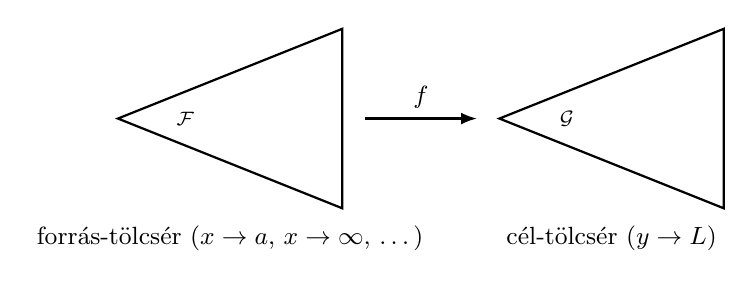
\begin{tikzpicture}[font=\small,scale=0.95]
  \draw[thick] (0,0) -- (3,1.2) -- (3,-1.2) -- cycle;
  \node at (0.9,0) {\scriptsize $\mathcal F$};
  \node[below] at (1.5,-1.3) {forrás-tölcsér ($x\to a$, $x\to\infty$, \dots)};
  \draw[nyil,thick] (3.3,0) -- node[above] {$f$} (4.8,0);
  \draw[thick] (5.1,0) -- (8.1,1.2) -- (8.1,-1.2) -- cycle;
  \node at (6.0,0) {\scriptsize $\mathcal G$};
  \node[below] at (6.6,-1.3) {cél-tölcsér ($y\to L$)};
\end{tikzpicture}
\end{center}

\subsection{A láncszabály mint funktorialitás}

A derivált „megőrzi a kompozíciót”: a pontbeli linearizálás funktor a differenciálható
függvények kategóriájából a lineáris leképezésekébe. A rajz ugyanaz a négyzet, amit a
fogaskerekes képnél láttunk --- csak most az alsó sor a lineáris közelítéseké.

\begin{center}
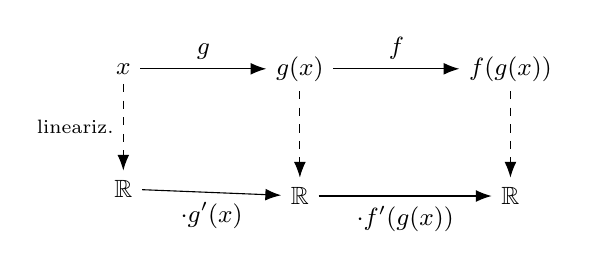
\begin{tikzpicture}[font=\small,node distance=16mm]
  \node (a) {$x$}; \node (b) [right=of a] {$g(x)$}; \node (c) [right=of b] {$f(g(x))$};
  \node (a2) [below=11mm of a] {$\R$}; \node (b2) [below=11mm of b] {$\R$}; \node (c2) [below=11mm of c] {$\R$};
  \draw[nyil] (a) -- node[above] {$g$} (b);
  \draw[nyil] (b) -- node[above] {$f$} (c);
  \draw[nyil] (a2) -- node[below] {$\cdot g'(x)$} (b2);
  \draw[nyil] (b2) -- node[below] {$\cdot f'(g(x))$} (c2);
  \draw[nyil,dashed] (a) -- node[left,font=\scriptsize] {lineariz.} (a2);
  \draw[nyil,dashed] (b) -- (b2);
  \draw[nyil,dashed] (c) -- (c2);
\end{tikzpicture}
\end{center}

\section{Melyik feladathoz melyik rajz?}

\begingroup
\small
\begin{longtable}{@{}p{2.2cm}p{5.0cm}p{7.6cm}@{}}
\toprule
\textbf{Gyakorlat} & \textbf{Ajánlott rajz} & \textbf{Mit olvasunk le róla} \\
\midrule
\endfirsthead
\toprule
\textbf{Gyakorlat} & \textbf{Ajánlott rajz} & \textbf{Mit olvasunk le róla} \\
\midrule
\endhead
\bottomrule
\endfoot
1.1, 1.3 & Venn-, Euler-diagram & jól definiáltság; halmazok egymásba ágyazása \\
1.2 & átlós tábla & az önhivatkozó sor lehetetlensége \\
1.4, 1.5 & gát/fal a számegyenesen & felső korlát vs.\ legkisebb felső korlát; egyértelműség \\
1.6 & felezéses szakaszrajz & részletösszeg $1-2^{-n}$; a határérték nem érhető el \\
1.7 & Venn + kvantorfa & implikáció mint tartalmazás \\
1.9 & Tennenbaum-négyzetek & végtelen leszállás, minimális nevező \\
1.10 & skatulyák a $[0,1)$ szakaszon & két pont egy rekeszben $\Rightarrow$ jó közelítés \\
1.11, 1.13 & számegyenes-távolság, vektorok & háromszög-egyenlőtlenség; „kerülő nem rövidebb” \\
1.12 & előjelvonal, tablófa & esetszétválasztás, tömör/üres pont \\
1.14, 1.15 & Gauss-téglalap, teleszkópos téglalapok & párosítás, becslés integrálképpel \\
1.16, 1.17 & lépcsőtornyok, teleszkóp & $3\sum i^2=(2n+1)\sum i$; nem indukciós út \\
1.18 & pókháló-diagram & fixpont, zsugorodási arány, csapdaintervallum \\
1.19 & rácsutak, Pascal-háromszög & utolsó lépés esetei; hokiütő-azonosság \\
2.1 & sávok metszete a számegyenesen & értelmezési tartomány mint szűrők metszete \\
2.2, 2.6 & vízszintes vonalteszt & injektív/szürjektív/bijektív \\
2.3--2.9 & tükrözés az $y=x$-re & inverz képlete, elvágási pontok, involúció \\
2.10--2.15 & nyíldiagram, kommutatív négyzet & kompozíció értelmezési tartománya; $\cos$-helyettesítés \\
2.16 & recept-fa + kontrollpont & transzformációk sorrendje és iránya \\
2.17--2.19 & ellenpélda-vázlat, gyöktényezős rajz & összeg/szorzat nem őrzi az injektivitást; fokszám és gyökszám \\
2.20 & előjelrajz gyöktényezőkkel & érintés vs.\ átmetszés; szélsőérték helye \\
3.1 & $\eps$--$\delta$ doboz, játékfa & a stratégia ($\delta = D(\eps)$) megkeresése \\
3.2, 3.3 & domináns tag, „messziről nézés” & három eset a fokszámok szerint; gyöktelenítés \\
3.4, 3.12 & lyukas grafikon & megszüntethető szakadás; a betöltendő érték \\
3.5, 3.6 & féloldali ágak & $|x|/x$ ugrás; féloldali határértékek \\
3.7 & egységkör-szendvics & $\sin x < x < \tan x$, rendőrelv \\
3.8, 3.9 & pólus + előjelvonal & $\pm\infty$ iránya oldalanként \\
3.10, 3.16 & hiperbola alatti terület & $\ln(1+t)$ becslése; $(1+1/n)^n$ monoton és korlátos \\
3.11 & teljes grafikonrajz & szakadástípusok, féloldali folytonosság \\
3.13 & illesztés & folytonosság mint egy egyenlet a paraméterre \\
3.14 & plafon-rajz & monoton + korlátos $\Rightarrow$ létező véges határérték \\
3.15 & sűrű fésű & racionálisokon egyező folytonos függvények \\
4.1 & szelő és érintő & differenciahányados határértéke \\
4.2 & fogaskerekek, kommutatív négyzet & láncszabály; szorzat- és hányadosszabály \\
4.3 & log-skála & relatív változás; szorzatból összeg \\
4.4--4.6 & négy „rossz pont” ikon & csúcs, függőleges érintő, cuspis, oszcilláció \\
4.7 & illesztés két feltétellel & érték \emph{és} meredekség egyezése \\
4.8 & négy alapikon + előjelvonal & teljes menetvizsgálat összefűzése \\
4.9 & gyanúsítottak bekarikázása & kritikus pontok, töréspontok, végpontok \\
4.10 & két linearizálás & L'Hospital képe; alkalmazhatóság ellenőrzése \\
4.11, 4.12, 4.14, 4.15 & geometriai vázlat + kényszer & egyváltozós redukció \\
4.13 & felezéses finomítás & diadikus arányok, majd folytonosság \\
\end{longtable}
\endgroup

\section{A rajzok pontos tartalma Leanben}

Minden alábbi tétel a \lean{RequestProject/Rajzok.lean} fájlban van, \lean{sorry} nélkül
bizonyítva. A táblázat így olvasandó: „ez az, amit a kép \emph{valóban} állít”.

\begingroup
\small
\begin{longtable}{@{}p{5.6cm}p{9.2cm}@{}}
\toprule
\textbf{Rajz} & \textbf{Lean-tétel} \\
\midrule
\endfirsthead
\toprule
\textbf{Rajz} & \textbf{Lean-tétel} \\
\midrule
\endhead
\bottomrule
\endfoot
átlós tábla (1.2) & \lean{atlos\_tabla} \\
Venn / De Morgan & \lean{venn\_de\_morgan}, \lean{venn\_tartalmazas} \\
tablófa: tagadás (3.1) & \lean{tablo\_nem\_hatarertek} \\
kvantorjáték, stratégia (3.1) & \lean{jatek\_strategia} \\
skatulyák (1.10 a) & \lean{skatulyaelv\_kozelites} \\
előjelvonal (1.12) & \lean{elojel\_vonal} \\
távolság-sáv (1.12 i) & \lean{tavolsag\_savban} \\
gát/fal (1.5) & \lean{ket\_fal\_egybeesik} \\
lépcsőtornyok (1.16) & \lean{negyzetszamok\_kepe} \\
Gauss-téglalap (1.14 a) & \lean{gauss\_teglalap} \\
vonaltesztek (2.2) & \lean{vizszintes\_vonal\_teszt}, \lean{szurjektiv\_vonal\_teszt} \\
tükrözés $y=x$-re (2.3) & \lean{grafikon\_tukrozes} \\
involúció szimmetriája (2.7) & \lean{involucio\_grafikon\_szimmetrikus} \\
pókháló (1.18) & \lean{pokhalo\_zsugorodas}, \lean{gyak\_1\_18} \\
egységkör-szendvics (3.7) & \lean{egysegkor\_szendvics}, \lean{rendorelv\_sav} \\
szelő $\to$ érintő (4.1) & \lean{szelo\_hatarerteke} \\
\end{longtable}
\endgroup

\section{Tíz rajz, amit érdemes fejből tudni}

\begin{enumerate}[nosep,leftmargin=*]
  \item \textbf{Sáv a számegyenesen}: $|x-a|<\eps$ (minden határérték-feladat alapja).
  \item \textbf{Előjelvonal} tömör/üres pontokkal (egyenlőtlenség, pólus, menetvizsgálat).
  \item \textbf{$\eps$--$\delta$ doboz} és a hozzá tartozó játékfa.
  \item \textbf{Fal-rajz} a $\sup$-hoz és a monoton korlátos plafonhoz.
  \item \textbf{Vízszintes vonalteszt} és a \textbf{tükrözés az $y=x$-re}.
  \item \textbf{Teleszkópos téglalapok} a görbe alatt (összeg becslése).
  \item \textbf{Egységkör-szendvics} a $\sin x/x$-hez.
  \item \textbf{Szelő $\to$ érintő} és a négy „rossz pont” ikon.
  \item \textbf{Pókháló} rekurzív sorozatokhoz.
  \item \textbf{Kommutatív háromszög/négyzet} kompozícióhoz és a láncszabályhoz.
\end{enumerate}

\bigskip
\noindent\textbf{Folytatás.} A bizonyítások \emph{lépésenkénti} felépítését --- milyen
építőkockákból állnak, és hogyan fűzzük őket össze --- a testvérfüzet tárgyalja:
\lean{kalkulus\_bizonyitas\_epitokockak.pdf}.

\end{document}
